\documentclass[german,oneside,color]{htldipl}
% Zulässige Class Options: 
%   Hauptsprache: german (default), english
%   Doppelseitig: oneside (default), twoside
%   Syntax-Highlighting: color (default), black

% die folgende Zeile einkommentieren für Arial-Ähnliche Schriftart
%\renewcommand{\familydefault}{\sfdefault}
\usepackage{hyperref}
\newcommand{\chapquote}[3]{\begin{quotation} \textit{#1} \end{quotation} \begin{flushright} - \footnotesize{#2, \textit{#3}\end{flushright} }}
\usepackage{spverbatim}
\usepackage{placeins}

\makeatletter
\newcommand\footnoteref[1]{\protected@xdef\@thefnmark{\ref{#1}}\@footnotemark}

\graphicspath{{images/}}    % Bilderverzeichnis

\usepackage[paper=a4paper,margin=3cm]{geometry}

\makeindex[title=Index]
\makeindex[name=allgemein, title=Allgemeiner Index]
\makeindex[name=name,title={Autoren Index}]
\makeindex[name=title,columns=1,title={Literatur Index}]
\indexsetup{level=\subsection*, toclevel=subsection, noclearpage}


\makeatletter
\@ifpackageloaded{biblatex_legacy}
  {\DeclareIndexNameFormat{default}{%
     \usebibmacro{index:name}{\index[name]}{#1}{#3}{#5}{#7}}}
  {\DeclareIndexNameFormat{default}{%
     \usebibmacro{index:name}{\index[name]}
       {\namepartfamily}
       {\namepartgiven}
       {\namepartprefix}
       {\namepartsuffix}}}
\makeatother

\DeclareIndexFieldFormat{indextitle}{%
  \usebibmacro{index:title}{\index[title]}{#1}}

\renewbibmacro*{bibindex}{%
  \ifbibindex
    {\indexnames{author}%
     \indexnames{editor}%
     \indexnames{translator}%
     \indexnames{commentator}%
     \indexfield{indextitle}}
    {}}

\makeatletter
\DeclareCiteCommand{\repeatfootcite}[\cbx@wrap]
  {\gdef\cbx@keys{}}
  {\xappto\cbx@keys{\thefield{entrykey},}}
  {}
  {\ifcsundef{cbx@lastin@\cbx@keys @\strfield{postnote}}
     {\csnumgdef{cbx@lastin@\cbx@keys @\strfield{postnote}}{-1}}{}%
   \ifsamepage{\value{instcount}}{\csuse{cbx@lastin@\cbx@keys @\strfield{postnote}}}
     {\footnotemark[\csuse{cbx@lastfn@\cbx@keys @\strfield{postnote}}]}
     {\xappto\cbx@cite{\noexpand\footcite%
        [\thefield{prenote}][\thefield{postnote}]{\cbx@keys}%
        \csnumgdef{cbx@lastfn@\cbx@keys @\strfield{postnote}}{\value{\@mpfn}}%
        \csnumgdef{cbx@lastin@\cbx@keys @\strfield{postnote}}{\value{instcount}}}}}

\newrobustcmd{\cbx@wrap}[1]{#1\cbx@cite\gdef\cbx@cite{}}
\def\cbx@cite{}
\makeatother

\makeglossaries
\loadglsentries{glossary}					%beinhaltet Daten für das Glossar
\addbibresource{literatur.bib}     %beinhaltet Daten für das


%%%----------------------------------------------------------
\begin{document}
%%%----------------------------------------------------------
%Einstellungen an die eigene Diplomarbeit anpassen

\title{Verteilerplanung}
\abteilung{IT}
%\schwerpunkt{} wenn kein Ausbildungsschwerpunkt vorhanden ist z.B. Informatik
\schwerpunkt{Computer Science}
\studienort{Wiener Neustadt}
\schule{HTBLuVA Wiener Neustadt}
\schullogo{htl.jpeg}
\abgabejahr{2020/21}
\betreuerA{Mag.\ Gabriele Haas}
\betreuerB{}
\betreuerC{}
%\betreuerD{} leer lassen wenn nicht vorhanden
\schuelerA{Christoph KRAUSE}
\evidenzA{5CHIF}
\subthemaA{Softwarearchitekturkonzepte, Optimierung von Workflow mittels BPMN und Usability, Datenaufbereitung in PDF-Format}
\schuelerB{David REINECKER}
\evidenzB{5CHIF}
\subthemaB{Graphische Benutzeroberfläche, Verfahren zur Gewährleistung der ÖNORM-Konformität}
\schuelerC{Christoph TEFFER}
\evidenzC{5CHIF}
\subthemaC{Datenbankerstellung, Backend-Funktionalitäten, Datensicherheit und Qualitätssicherung}
\schuelerD{}
\evidenzD{}
\subthemaD{}
\schuelerE{}
\evidenzE{}
\subthemaE{}
%\schuelerE{} leer lassen wenn nicht vorhanden
%\evidenzE{}
%\subthemaE{}

%%%----------------------------------------------------------
\frontmatter
\maketitle
\tableofcontents
%%%----------------------------------------------------------

%\chapter{Vorwort}

Dies ist \textbf{Version \htldiplDate} der \latex-Dokumentenvorlage für 
die Diplomarbeiten an der HTL Wiener Neustadt, basierend auf der
Vorlage für Abschlussarbeiten an der FH Hagenberg erstellt von Dr.\ Wilhelm
Burger\footnote{\url{http://www.fh-hagenberg.at/staff/burger/diplomarbeit/}}.

Die Verwendung dieser Vorlage ist jedermann freigestellt und an
keinerlei Erwähnung gebunden. Allerdings -- wer sie als Grundlage
seiner eigenen Arbeit verwenden möchte, sollte nicht einfach
("`ung'schaut"') darauf los werken, sondern zumindest die
wichtigsten Teile des Dokuments \emph{lesen} und nach Möglichkeit
auch beherzigen. Die Erfahrung zeigt, dass dies die Qualität der
Ergebnisse deutlich zu steigern vermag.

Der Quelltext zu diesem Dokument sowie das zugehörige
\latex-Paket sind in der jeweils aktuellen Version online
verfügbar unter
%
\begin{quote}
\url{https://github.com/wschermann/Diplomarbeitsvorlage}
\end{quote}
%
Trotz großer Mühe enthält dieses Dokument zweifellos Fehler und Unzulänglichkeiten
-- Kommentare, Verbesserungsvorschläge und passende Ergänzungen
sind daher stets willkommen, am einfachsten per E-Mail direkt an mich:
\begin{center}%
\begin{tabular}{l}
\nolinkurl{w.schermann@htlwrn.ac.at} \\
Wolfgang Schermann MSc \\
HTL Wiener Neustadt -- Informatik\\
Austria
\end{tabular}
\end{center}

\noindent
Übrigens, hier im Vorwort kann man kurz auf die Entstehung  des Dokuments eingehen.
Hier ist auch der Platz für allfällige Danksagungen (\zB an den Betreuer, 
den Begutachter, die Familie, den Hund, ...), Widmungen und philosophische 
Anmerkungen. Das sollte man allerdings auch nicht übertreiben und sich auf 
einen Umfang von maximal zwei Seiten beschränken.




				%ggfs. weglassen
%%Inkludiert die 4. vorgeschriebenen Seiten an Dokumentation aus dem gedruckten PDF-Formular
%Das Formular erst vor der Abgabe vollständig ausfüllen, da z.B. das Bild zur Diplomarbeit vorher nicht vorhanden sein wird
\begingroup
\makeatletter
\newpage
\@twosidefalse
\includepdf[pages=1-1,pagecommand={\chapter[Diplomarbeit Dokumentation]{}}]{pdf/eingebundene_details.pdf}
\includepdf[pages=2-2,pagecommand={\thispagestyle{plain}}]{pdf/eingebundene_details.pdf}
\includepdf[pages=3-3,pagecommand={\chapter[Diploma Thesis Documentation]{}}]{pdf/eingebundene_details.pdf}
\includepdf[pages=4-4,pagecommand={\thispagestyle{plain}}]{pdf/eingebundene_details.pdf}
\endgroup
%\chapter{Kurzfassung}

Im Jahr 2019 hat die Europäische Union im Rahmen von Erasmus+ die Finanzierung des Projekts KA229-71D8817F eingewilligt. Die fünf teilnehmenden Staaten haben seitdem mit der Umsetzung begonnen. Ziel ist die Erschaffung und Etablierung eines virtuellen Museums. In Österreich steuert die HTBLuVA Wiener Neustadt (HTLWRN) einen signifikanten Teil zu der technischen Realisierung bei. Diese Diplomarbeit stellt den Grundstein für weitere Entwicklungen in den Folgejahren dar und untersucht unterschiedlichste Aspekte für die schlussendliche Implementierung.

Der größte Schwerpunkt in dieser Arbeit liegt bei dem ausführlichen Testen, Untersuchen und objektiven Bewerten von zahlreichen Softwarelösungen zur Entwicklung eines virtuellen Museums. Schlussendlich grenzen wir aus einer Vielzahl von Realisierungswerkzeugen die zwei geeignetsten ein, und überprüfen die tatsächliche Eignung in Abhängigkeit von definierten Kriterien. Wir erwarten uns somit, die finale Implementierung für zukünftige Entwickler erheblich zu erleichtern und zum Erfolg des Projekts beizutragen.

Aufgrund von zeitlichen Problemen ist in dieser Schrift nur der erste Teil der Diplomarbeit verfasst. Der Zweite wird im September 2020 folgen und beinhaltet die eigentliche Softwareevaluierung.	
%\chapter{Abstract}

In 2019, the European Union agreed to finance the KA229-71D8817F project under Erasmus+. Since then, the five participating countries have started to implement the project. The aim is to create and establish a virtual museum. In Austria, the HTBLuVA Wiener Neustadt (HTLWRN) is making a significant contribution to the technical implementation. This diploma thesis lays the foundation for further developments in the following years and examines different aspects for the final implementation.

The main focus of this work is the extensive testing, analysis and unbiased evaluation of numerous software solutions for the development of a virtual museum. Finally, we narrow down the two most suitable toolkits from a variety of alternatives and check the actual suitability depending on defined criteria. We expect to facilitate the final implementation for future developers and contribute to the success of the project.

Due to scheduling difficulties, only the first part of the thesis is published in this paper. The second part will follow in September 2020 and contains the actual software evaluation.			

%%%----------------------------------------------------------
\mainmatter           %Hauptteil (ab hier arab. Seitenzahlen)
%%%----------------------------------------------------------

%\include{einleitung}
\chapter{Datenbanken}
\label{cha:Datenbankerstellung}
\begin{flushleft}

Hinter, so gut wie jeder, Software steht eine Datenbank. Dieses Kapitel beschäftigt sich mit dem Erstellen einer relationales Datenbank. Dazu gehört die Erklärung des Konzepts der relationalen Datenbank, das Erstellen eines Datenmodells inklusive der Begriffe und Konzepte. 

\section{Was ist eine Datenbank im Allgemeinen}
 
 Im Allgemeinen ist eine Datenbank ein Ort an dem Daten abgespeichert sind. Diese Daten werden nur von einer bestimmten Gruppe von Benutzern benutzt und die Daten haben einen gewissen Zweck und Zusammenhang. 
 
 \section{Datenbankmanagementsystem (DBMS)}
 
 Ein DBMS ist eine Software, die dabei hilft Datenbanken zu verwalten. Somit wird den Benutzer das Erstellen, Bearbeiten oder Löschen einer Datenbank erleichtert. Außerdem hat ein DBMS viele andere Aufgaben. Eine oder mehrerer Datenbanken bilden in Verbindung mit dem Datanbankmangementsystem das Datenbanksystem.
 
 \subsection{Aufgaben eines DBMS}
 
 Ein DBMS muss alle Daten einheitlich verwalten und somit jedes einzelne logische Datenelement an genau einem Ort abspeichern. Das DBMS muss aber die Vielzahl der komplexen Beziehungen in der Datenbank definieren  und zusammenhängende Daten rasch miteinander verknüpfen können.
 
 Neben der Datenverwaltung muss das DBMS auch noch eine Schnittstelle einer Datenbanksprache, in den meisten Fällen SQL (Strucured Query Language), für: 
\begin{itemize}
\item Datenanfragen, Datenmanipulation (Data Manipulation Language, DML
\end{itemize}
\begin{itemize}
\item Verwaltung der Daten (Data Definition Language, DDL)
\end{itemize}
\begin{itemize}
\item Berechtigungssteuerung (Data Controll Language, DCL)
\end{itemize}
 
 Durch den Einsatz von einem DBMS kann man den unautorisierten Zugriff auf Daten innerhalb der Datenbank verhindert werden. Das ist sehr wichtig, weil sensible Daten abgespeichert werden können.
 
Ein DBMS verwaltet ebenfalls die Benutzer. Sollten mehrere Benutzer gleichzeitig auf der Datenbank arbeiten und auf die selben Daten zugreifen, kann das zu einem Schreibkonflikt führen.

Es wird auch erwartet,dass nach auftreten Hard- oder Softwarefehlern die Datenbank wieder in einen korrekten und vollständigen Zustand ist.  

\section {Architektur eines Datenbanksystems}

Architektur kann im Bereich der Datenbankanwendungen einen unterschiedlichen Kontext haben. Man unterscheided grundsätzlich zwischen:
\begin{itemize}
    \item Systemarchitektur eines Datenbankmanagementsystems
\end{itemize}
\begin{itemize}
    \item Schemaarchitektur eines Datenbanksystems
\end{itemize}
\begin{itemize}
    \item Anwendungsarchtitekturs
\end{itemize}
\begin{itemize}
    \item Verteilte Architektur
\end{itemize}

 Doch mit dem Begriff Architektur ist oftmals die Schnemaarchitektur gemeint.

\subsection{Datenbankschema}

Jedes Modell(->x.x.x), welches ich für die Datenbank erstelle, sollte immer zwischen der Beschreibung der Struktur und des Inhalts der Datenbank unterscheiden.

Die Strukturelle Beschreibung bezeichnet man als Datenbankschema. Dieses Schema versucht man mit der Data Definition Language umzusetzen.Die grafische Darstellung wird Schemadiagramm genannt.
So ein Datenbankschema kann für jede Anwendung spezifisch angelegt werden. Doch es gibt auch noch ein vordefiniertes Schema, für eine bestimmte Kategorie von Anwendungen, Web-Anwendung, Desktopanwendung usw., welche man als Referenzmodell bezeichnet. Solche Referenzmodelle unterliegen Standarts, erleichtertn den Austausch von Daten und verringern die Zeit die zum Entwicklung der Datenbankanwendung benötigt wird. 

Daten die zu einem bestimmten Zeitpunkt in der Datenbank abgespeichert wurden, werden als Datenbankzustand bezeichnet. Jede Änderung der Datenbank entspricht einen neuen Datenbankzustand. Ziel ist es das dieser Datebbankzustand konstant ist. Ein Datenbankzustand gilt als konstant, wenn alle Daten vollständig vorhanden sind. 
Jeder Datensatz der abgespeichert wird stellt eine Instanz dar. Eine Instanz entspricht einen Objekt oder auch Entity (->x.x.x) genannt.
Der Datenbankzustand wird als Extension bezeichnet das Schema als Intension und die Veränderung Schemas heißt Schemaevolution.

\subsection{Drei-Schichten-Architektur}

Der Grundlegende Aufbau des Datenbanksystems wird durch die Drei-Schichten-Architektur beschrieben. Ziel dieses Modells ist es die, physische (interne), konzeptionelle (logische) und die externe Schicht zu trennen. 
Jede dieser Schichten verfolgt den Zweck die abzuspeichernden Daten strukturiert abzuspeichern und die dem Anwender wieder zu Verfügung zu Stellen. Für den Datenaustausch dieses Schichten werden Transformationsregeln definiert. Der Aufbau ist für die Einhaltung der Anforderungen an das Datenbanksystem extrem wichtig. 

\subsubsection{physiche Schicht}

In dieser Schicht werden die physischen Speicherstrukturen und Zugriffsmechnismen einer Datenbank beschrieben.

Dafür wird ein der Ebene ein Schema für die Speicherung von Daten und deren Verwaltung implementiert.

Auf dieser Ebene wird die Art und Weise der Datenspeicherung beschrieben. Die Festlegung werden bei der Realisierung des physischen Modells (->x.x.x).

\subsubsection{konzetuelle Schicht}

Diese Schicht dient dazu, die logische Struktur dar. Anders gesagt sind hier die für den Nutzer relevanten Daten abgespeichert. 
Hier handelt es sich um die Beschreibung der Daten und deren Zusammenhänge. Auf Basisis des konzepionellen Schemas (->x.x.x) werden den externen Schemas Datenausschnitte zu Verfügung gestellt

\subsubsection{Externe Schicht}

In dieser Schicht befinden sich mehrere Sichten für Benutzer. Jede dieser Sichten repräsentiert eine Gruppe von Anwendern, die Aufgrund derer Eigenschaften einen Teil der hinterlegten Daten sehen. 
Der Rest der und das komplette Datenmodell der logischen Schicht sind den Anwender aber verborgen. Dadurch wird erreicht, dass jeder Benutzer nur das sieht, das ihm betrifft. Der Anwender kann auf die logische Schicht nicht zugreifen.

\subsection {Datenunabhängigkeit}

Dieses Prinzip beschreibt auf welche Daten der Datenbank ein Benutzer zugreifen darf. Außerdem hat der Entwickler die Möglichkeit das Schema auf einer Ebene zu ändern ohne das Schema der nächst höheren Schicht ändern zu müssen. Auch hier gibt es wieder die logische- und physische Datenunabhängikeit.

\subsubsection{logische Datenunabhängikeit}

Hier kann ich das konzeptionelle Schema verändern ohne das Externe zu ändern, außer für eine Änderung an der Datenbankstruktur betroffenen externen Schemata müssen, die Schichtendefinitionen angepasst werden. So kann zum Beispiel ein Attribut geändert werden, ohne dass das eine Auswirkung auf die externe Schicht hat.

\subsubsection{Phyische Datenunabhängigkeit}

Bei einer Änderung des internen Schemas hat das wieder keine Auswirkung auf das konzeptuelle- und das externe Schema. Netztwerkaritige Datenbanken können keine physische Datenunabhängigkeit bieten, weil diese starke Bindungen an Zugriffspfade haben.

\section{Datenbank Konzepte}

Es gibt verschiedene Arten von Datenbank Konzepten. Diese unterscheiden sich vor allem durch ihre Struktur. Zu den beliebtesten Konzepten gehören
\begin{itemize}
    \item NoSQL-Datenbanken
\end{itemize}
\begin{itemize}
    \item Objektrelationale
\end{itemize}
\begin{itemize}
    \item relationale Datenbanken
\end{itemize}
\break

\subsection{NoSQL-Datenbanken}

NoSQL steht für Not-Only-SQL (structured Query Language) und nicht wie man vermuten könnte, dass sie kein SQL unterstützen. Diese Art der Datenbank wird vor allem in der Web-Entwicklung verwendet. Datenbankmanagementsysteme müssen viel größere Datenmengen verarbeiten und kommen vor allem im Web Bereich oft in unstrukturierter oder semi strukturierter Form vor.
Unstrukturiert bedeuten, dass die Daten sind in einen nicht formalisierbaren Form vorliegen, dass heißt man kann sie nicht wirklich identifizieren. Textdokumente, Viedos oder Bilder sind gute Beispiele für unstrukturierte Daten. 
Semi Strukturierte Daten sind Daten, die nicht wirklich in einer Struktur vorliegen aber einen Teil der Strukturinformation mit sich tragen.

NoSQL-Datenbanken haben kein bzw. ein schwaches Schema und ist von Anfang an auf horizontale Skalierbarkeit ausgerichtet. Das heißt die Anzahl der Recheknoten in einer verteilten Datenbank wird erhöht.

NoSQLDatenbank ist nicht gleich NoSQL.
Man unterscheidet zwischen:
\begin{itemize}
    \item Key-Value-Datenbanksystemen
\end{itemize}
\begin{itemize}
    \item dokumentorientierte Datanbanksystemen
\end{itemize}
\begin{itemize}
    \item Column-Family-Datenbanksystemen
\end{itemize}

\subsubsection{Key-Value-Datenbanksysteme}

Wie der Name schon vermuten lässt, speichert die Datenbank die Daten in Form von Key-Value, bzw. Schlüssel-Wert Paaren ab. Der Schlüssel muss eindeutig sein. Die Eindeutigkeit eines solchen Schlüssels kann sich auf die ganze Datenbank oder einen Namensraum innerhalb der Datenbank beziehen. Der Value kann beliebige Daten abspeichern. Den Datenbanksystem ist es egal welche Struktur die Daten haben. Zudem hat das Datenbanksystem auch keine Kenntnisse über den Dateninhalt der Values.

Da solch ein Datenbanksystem kein Schema hat, bietet es die größtmögliche Flexibilität beim Schema der abzuspeichernden Daten. Auf der Kehrseite wird das Management der Schema-Evoulution gar nicht unterstützt.

Auslesen kann man solche Schlüssel-Wert Paare indem man den Schlüssel oder einen Schlüsselbereich angibt. Aus Gründen der Effizienz werden den Schlüssel vom System mit einem B-Baum-Index oder einem Hash versehen. (soll ich erklären was das ist?)
Zugriffe auf die Struktur sind unmöglich, weil, wie bereits erwähnt das Datenbanksystem keine Informationen über Struktur und Inhalt der Values hat. Aus diesem Grund kann man Key-Value-Paare auch nicht werte-basiert miteinander verknüpfen.

Key-Value-Paare können auch nur eingefügt oder gelöscht werden, Veränderungen sind nicht möglich.

Diese Datenbanksysteme eignen sich gut für Anwendungen, die aus einer großen Menge von Daten einen Key selektieren oder abspeichern möchten. Speicherung von Nutzerprofilen und Warenkorbdetails sind gure Beispiele.

\subsubsection{dokumentenorientierte Datenbanksysteme}

Auch hier werden die Daten wieder in Key-Value-Paaren gespeichert. Der große Unterschied ist, das hier Dokumente in strukturierter Form und in einem bestimmten Format abgespeichert werden. Die typisch verwendeten Datenformate sind JSON, XML oder BSON, die binäre Version von JSON (Soll ich diese 3 Formate erklären). Diese drei Formate haben eines gemeinsam, sie sind eine Folge von \textbf{Property-Value-Paaren} darstellen. Eine Property ist ein identifizierender Bezeichner der in einigen Formaten innerhalb eines Dokuments eindeutig sein muss und gegebenenfalls auch mehrwertig sein kann. Values können auch Properties enthalen, somit ist eine hierachische Architektur möglich.

Die Struktur der Daten muss nicht im Vorhinein deklariert werden und kann zwischen den Dokumenten variieren. Dokumente die sich in ihrer Struktur stark unterscheiden speichert man am besten getrennt in \textbf{Collections} ab. Ähnlich strukturierte Dokumente speichert man am Besten in der selben Collection ab.

Dokumente werden geziehlt anhand der Properties der Dokumente ausgewählt. Einige Systeme übernehmen die Indizierung der Properties selbst in die Hand. Verknüpfen kann man die Dokumente auch hier nicht. Bei Bedarf kann man das aber durch mehrere Abfragen realsieren. 
Dokumente können auch hier komplett gelöscht oder eingefügt werden. In den meisten dokumentorientierten Datanbanksystemen ist auch möglich einzelne Properties in einem Dokument zu ändern,löschen oder einzufügen.

Einsatz finden solche Datenbanksysteme vor allem bei Anwendungen die eine sehr große Datenmenge strukturierter oder semi-strukturierter Daten verarbeiten sollen und gegebenenfalls Schemaflexibilität benötigen. Blogging-Plattformen verwenden diese Datenbanksysteme gerne.

\subsubsection{Column-Family-Datenbanksysteme}

Daten werden hier in einer oder mehreren Tabllen gespeichert. Die Datensätze werden dann in Zeilen modeliert, welche durch einen eindeutigen Schlüssel, der aus einem oder mehreren Werten bestehen kann, identifiziert werden können. Jeder dieser Datensätze kann mehrere Attribute besitzen, die durch Spaltenbezeichner ausgezeichnet werden. Diese Spalten werden in eine Spaltenfamilie (Column family) gruppiert. Eine spezifische Spalte wird durch die Angabe des Bezeichners der Spaltenfamilie, der Tabelle und der Spalte qualifiziert. Spaltenfamilien können zur logischen Gruppierung der Spalten als auich zur phyischen Optimierung verwendet werden. 
Im Gegensatz zu Spalten müssen Spaltenfamilien je nach System bereits beim Erstellen der Tabelle definiert worden sein. Spalten können zu jederzeit hinzugefügt werden, aber nicht unbedingt durch Schemaänderungen. Fügt man einen neuen Datensatz mit einer zusätzlichen Spalte ein, wird das erkannt und eine neue Spalte angelegt. 
Im Gegensatz zur relationalen Datenbank werden die Daten nicht zeilenweise sonder spaltenweise gespeichert. Diese Technik findet auch beim Data-Warehouse seinen Einsatz. Durch das spaltenweise Speichern garantiert man die Schemaflexibilität. Außerdem werden Datensätze bei Veränderung in eine neue Version gespeichert und mit einem Timestamp versehen. 

Column-FAmily-Datenbanken unterstützen die Auswahl von Daten anhand des Schlüssels oder den in der Spalte gespeicherten Werts. Unter Verwendung eines Timestamps können auch verschiedene Versionen der Daten aufgerufen werden.  Die Art des Zugriffs ist dabei von System zu System unterschiedlich. Teilweise werden SQL-ähnliche Abfragesprachen verwendet, teilweise Interfaces mit Scan- und Filter-Operatoren. Indexierung wird im Normalfall unterstützt. Verknüpfungen mittels Join-Operationen werden auch hier nicht unterstützt und müssen bei Bedarf in der Anwendung programmiert werden. 
Nebn vollständigen Einfügen- und Löschen, wird auch hier adas partielle Update unterstützt, d.h. ich kann den Wert einer bestimmten Spalte ändern. 













\subsubsection{Grundbegriffe}

Wie schon der Name verrät ist das zentrale Element der relationalen DB die Relation. Eine Relation sieht aus wie eine Wertetabelle, bei der die Reihen als Tupel und die Spalten als Attribute bezeichnet werden. 

Ein relationales DB-Schema besteht aus einer Menge von Relationenschemata. Aus diesen Schema kann man die jeweiligen Relationen ableiten. Das Beschreiben eines solchen Schemas ist auf die Datenstruktur begrenzt. 
Zur Beschreibung dieser Datenstruktur werden Attribute, Wertebereich, Relationen und Tupel verwendet.


\chapquote{"Ein Attribut repräsentiert eine Eigenschaft eines Objekttyps und wird über eine Tabellenspalte abgebildet"
}{\citeauthor{Prof. Dr. Petra Sauer}}{\citetitle{HANSER Taschenbuch Datenbaken S.68}}

Wertebereiche werden auch als Domänen bezeichnet und enthält die Menge von möglichen Werten des Attributes. Dazu werden auch Standartdatentypen wie Integer (Ganzzahliger werd), String (Zeichenkette), Date (Datum) etc. abgebildet. 

Eine Relation ist eine endliche Menge von Attributen und deren Domänen. Relationen sind Ausprägungen oder Zustände des Relationenschemas. Das Relationenschema ist die Intention und die Relation ist die Extension. Die Relation die aktuell als Ausprägung eines Relationalschemas vorhanden ist, wird als Basisrelation bezeichnet Ein Relationenschema mit einer Attribut Menge wird so dargestellt: R(A1, A2, ..., An). Durch den Anzahl der Attribute wird der Grad der Relation bestimmt. Hat also eine Relation zum Beispiel 5 Attribute hat diese den Grad 5.  Die einzelnen Objekte die durch Elemente der Relation definiert werden, nennt man Tupel. 

Relationen haben gewisse Eigenschaften oder besser gesagt Regeln an die man sich halten muss. J

\section{Datenmodellierung} \label{Datenmodell}


Ein Datenmodell beschreibt die Informationen in einer Datenbank.Ziel des Modells ist es der Datenbank Struktur zu verleihen. In Sinne des Drei-Schichten-Konzepts muss ich ein physisches, ein logisches und ein konzeptionelles Schema erstellen. Die Schemata müssen in einer gewissen Reihenfolge entwickelt werden und führen von einer abstrakten zu einer konkreten Beschreibung. 

\subsection{Ablauf} 
Das Entwickeln bzw. das Entwerfen einer Datenbank orientiert sich stark an den Entwurfsschritten des Phasenmodells. Die Phasen sind an die Bedürfnisse des Datenbankentwurfes angepasst. Phase 1 ist die Anforderungsanalyse, Phase 2 ist der Entwurf des konzeptionellen Schemas, Phase 3 der logische Entwurf, Phase 4 beschäftigt sich mit der Definition der Daten, Phase 5 der physische Entwurf und Phase 6 ist die Implementierung und Wartung der Datenbank.

\subsubsection{Anforderungsanalyse}
In dieser Phase der Entwicklung beschafft man sich die nötigen Informationen die für die Datenbank realevant sind. Diese relevanten Informationen werden nun zu Anforderungen. Man Unterscheidet zwischen Informations- und Bearbeitungsanforderungen. 
\chapquote{"Informationsanforderungen werden im Rahmen der Datenanalyse erfasst und beschreiben die Daten unabhängig von der Auswertung"
}{\citeauthor{Prof. Dr. Petra Sauer}}{\citetitle{HANSER Taschenbuch Datenbaken S.45}}
Der Datenbank-Entwurf basiert auf den Informationsanforderungen
\chapquote{"Bearbeitungsanforerungen werden im Rahmen der Funktionsanalyse erfasst und beschreiben die Auswertungs- und Bearbeitungserfordernisse auf der DB"}{\citeauthor{Prof. Dr. Petra Sauer}}{\citetitle{HANSER Taschenbuch Datenbaken S.45}}

Die Bearbeitungsanforderungen beinhalten die Angaben über die Art des zu bearbeitenden Prozesses, damit sind Abfragen, Updates oder Berichtsgenerierung gemeint. Quantität, zum Beispiel Häufigkeit eines Prozesses, des aufzuführenden Prozesses zählen auch zu den Angaben für die Bearbeitungsanforderungen. Außerdem sollten hier auch schon Sicherheitsanforderungen, zum Beispiel Zugriffsrechte, an die Datenbank definiert sein. In der Funktionsanalyse wird analysiert wie sich das System verhalten soll und wie man dieses Verhalten erreichen kann.

\subsubsection{Konzeptioneller Entwurf}
\chapquote{Datenbanken stellen eine abstrahierendes Abbild der Realität dar}{\citeauthor{Prof. Dr. Petra Sauer}}{\citetitle{HANSER Taschenbuch Datenbaken S.46}}

Nach der Anforderungsanlyse wird in dieser Phase der sogenannte "Abzubildender Weltauschnitt", auf englisch "Universe of Disource", zum ersten Mal formal beschrieben. Zu Beachten ist, dass man hier noch nicht versucht das Ganze in einem konkreten Datenbank Management System zu realisieren, weil diese Beschreibung eine gute Basis für die weiteren Schritte beim Entwickeln eines Systems sein soll.

Um die Datenbank formal zu beschreiben wird ein Datenmodell, wie zum Beispiel das Entity-Relation-Modell (ERM) verwendet. Die Anforderungen des Benutzers werden in einer formalen Schreibweise dokumentiert, daraus ergibt sich das konzeptuelle und die externen Schemata.

Für die Entwicklung solcher Schemata gibt es zwei Ansätze, nämlich den Top-Down-Ansatz, bei den zuerst das konzeptuelle Schema modelliert und externe Schemata werden als nicht notwendige Ausschnitte des konzeptuellen Schemas abgeleitet. Beim Bottom-Down-Ansatz wird zuerst das externe Schema modelliert, aus deren Integration das konzeptuelle Schema besteht. Das externe Schema gibt Einsicht über die Anforderungen einzelner Benutzer wieder. Aufgrund, dass diese unterschiedliche Anforderungen stellen kann es zu Überschneidung und Widersprüche kommen. Bevor man die einzelnen Schemata integriert sollte man diese analysieren und Konflikte erkennen und auflösen. Konflikte können zu Redundanzen (gleicher Speicherinhalt) oder einen inkonsistenten(nicht vollständigen) Datenbestand führen. Zu den Konflikten gehören der Namenskonflikt, tritt bei Namensüberschneidungen oder Ähnlichkeiten durch Sonderzeichen auf, der Typkonflikt, wenn verschiedene Datenstrukturen das selbe Element, basierend auf unterschiedlichen Aussagen diverser Benutzer zum abzubildendem Weltauschschnitt, Strukturkonflikt, wenn verschiedene Modelierungsvarianten zu einem Sachverhalt und zum Schluss noch der Bedingungskonflikt, welcher durch die Verwendung von verschiedenen Integritätsbedingungen in Schichten auftreten kann.

\subsubsection{Logischer Entwurf}

Hier wird auf Basis des konzeptuellen Schemas die Datenstruktur weiter formell beschrieben, aber in einem anderen Beschreibungsformulismus.

\chapquote{Das logische Schema beschreibt die Datenstruktur des Universe of Discourse in Abhängigkeit vom konkreten Datenmodells des DBMS}{\citeauthor{Prof. Dr. Petra Sauer}}{\citetitle{HANSER Taschenbuch Datenbaken S.47}}

In diesem Schritt wird auch entschieden ob man die Datenbank in einem konventionellen, objektorientierten, objektrelationalen oder einem relationalen DBMS realisieren möchte. Meistens wird man sich aber für ein relationales DBMS entscheiden. Außerdem wird hier die Vorarbeit für das Modelierungskonzept der Anwendung. 
Zwei Schritte sind nötig um ein logisches Schema zu entwickeln. Zuerst wird das konzeptuelle Schema auf ein logisches Schema transformiert. Hier zahlt sich ein realtaionles DBMS aus, weil dieser Schritt kann automatisiert werden, weil sich ein System von Regeln der Transformationen, auf welche ich in einem späteren Kapitel näher eingehen werde, etabliert hat. Im nächsten Schritt geht es darum das logische Schema zu Verbessern oder zu Bearbeiten. Wichtig ist es vor allem Redundanzen zu minimieren, wenn nicht sogar zu vermeiden. Sollte man sich für das relationale DBMS entschieden haben, folgt nun die Normalisierung, auf welche ich in einem späteren Kapitel detaillierter beschreiben werde. Die Normalisierung ist ein Verfahren um ein relationales DBMS so zu gestalten, dass sich der Datenbestand nach Einfüge-, Änderungs- und Löschoperationen wieder in einen konsistenten Zustand befindet. Dazu teilt man Redundanzen immer wieder in Relationen auf um diese schrittweise zu minimieren.

Abbildung logisches relationales Datenmodell

\subsubsection{Datendefinition}

In dieser Phase wird mit Hilfe der Datenbanksprache, meistens SQL die logischen und externen Schemata beschrieben. Die logischen Schemata werden mithilfe der Data Definition Language (DDL) beschrieben und die verschiedenen Sichten mit der View Definition Language (VDL), welche ein Teil der DDL ist.  Die DDL hilft dabei bei einem relationalen Datenmodell Relationen, Wertebereich und Attribute zu definieren.

Neben der Datenbankstruktur werden in dieser Phase auch die Integritätsbedingungen mit der Datenbanksprache beschrieben, ein wichtier Teil ist es die Fremd und Primärschlüssel richtig zu setzen. Das Ergebnis dieser Phase ist ein Datenbankschemata für das konkrete DBMS

\subsubsection{Physischer Entwurf}

Hier geht es darum ein internes Schema zu entwickeln, dabei hilft uns die Stroage Structure Language (SSL). Um dieses Schema zu entwickeln muss man die geeigneten Speicherform und mögliche Zugriffspfade der Daten zu definieren.

Ziel des Ganzen ist es eine hohe Leistung der Datenbank zu gewährleisten, dazu gehören geringe Zugriffszeiten, die optionale Nutzung des Speicherplatzes und eine hohe Durchsatzrate. Hier wird quasi die Definition der Datenbank optimiert

\subsubsection{Implementierung und Wartung}

Ist die Datenbank schlussendlich installiert, dort wo sie für den Dauerbetrieb entwickelt wurde endet die Entwurfsphase. Dazu gehört das Erfassen oder Generieren von Datenbeständen, dazu benötigt man die Data Manipulation Language (DML) des DBMS. Bei Übernahme eines anderen System kommt es oft zu Migrationsproblemen. Um dieses Problem zu bewältigen sollte man die Datenstrukturen abgleichen und möglicherweise muss man ein Kovertierungsprogramm erstellen.

Sobald die Datenbank in den Betrieb aufgenommen wird beginnt die Wartungsphase. Da man möchte, dass eine Datenbank so lange wie möglich genutzt werden kann, muss man diese laufend an neue Anforderungen anpassen, zum Beispiel könnte der Kunde etwas an seiner IT-Struktur ändern oder es muss etwas am Datenmodell geändert werden.




\subsubsection{ERM}
Wie schon vorher erwähnt verwendet man ein ERM um eine Datenbank das erste Mal formal zu beschreiben. Es wird eingesetzt um das konzeptuellen Schemas zu entwerfen und zum Modellieren der Benutzersichten(Views).
Das ERM ist ein semantisches Datenmodell.

\chapquote{Semantische Datenmodelle beschreiben einen Weltauschnitt als Menge von Gegenständen (Objekten), zwischen den wohldefinierte Beziehungen existieren und die durch Eigenschaften charakterisiert werden.}{\citeauthor{Prof. Dr. Petra Sauer}}{\citetitle{HANSER Taschenbuch Datenbaken S.49}}

Aufgrund seiner Unabhängigkeit eines konkreten DBMS, seiner guten Übersicht, der Beschränkung auf wenige und einfache Basiskonzepten und der Möglichkeit des uneingeschränkten entwickelns eines Datenmodells hat sich das ERM durchgesetzt.

\subsubsection{Grundkonzept}

Ein ERM enthält Entities, Entitytypen, die Beziehungen oder Realationships, Beziehungs- beziehungsweise Realtionshiptypen, Attribute, Werte sowie Rollen.
Grafisch wird ein ERM als Entity-Realtion-Diagramm (ERD) dargestellt. Zum allgemeinen Verständnis werden ich immer wieder Beispiele bringen. Zu Beginn gleich mal ein Standartbesipiel nämlich Lieferant und Artikel. In der unteren Abbildung kann man eine ganz einfache Beziehung, zwischen den Entitytypen Artikel und Lieferant sehen


Abbildung Lieferant liefert Artikel  


\chapquote{Ein Entity ist ein abgrenzbarer, selbständiger Gegenstand, ein Begriff, ein Ding, eine Person oder auch ein Ereignis des zu Modellierenden Weltauschnschnitts.}{\citeauthor{Prof. Dr. Petra Sauer}}{\citetitle{HANSER Taschenbuch Datenbaken S.51}}

Entities werden nicht einzeln dargestellt, sondern in einer Menge des dazugehörigen Entityps. In unserem Beispiel sind Lieferant und Artikel unsere Enities. Zwischen den Entities werden Beziehungen verknüpft. Entities werden über Werte oder Attribute näher beschrieben

\chapquote{Eine Beziehung ist die logische Verknüpfung von zwei oder mehreren Entities.}{\citeauthor{Prof. Dr. Petra Sauer}}{\citetitle{HANSER Taschenbuch Datenbaken S.51}}
Genau wie bei den Enteties werden Beziehungen nicht einzeln dargestellt sondern auch wieder durch Mengen des dazugehörigen Beziehungstyps, weil man sonst die Übersicht verlieren würde.

Entities werden meistens als Rechteck dargestellt, deren Attribute als Ellipsen und Beziehungen meistens als Rauten. Attribute werden aber meistens aus Gründen der Übersicht meistens nicht dargestellt.
Enteties eines Entitytypen haben in Beziehungen immer eine gewisse Funktion, welche als Rolle bezeichnet wird über eine Beschriftung des Beziehungstypen am Ende der Kante dargestellt. Beziehungstypen werden quantitativ beschrieben. Ein klassisches ERD beschreibt die Beziehungstypen in der MinMax-Notation. Die Aussage eines ERD in der MinMax-Notation ist, wie viele Entities maximal mit wie vielen anderen Entities eines anderen Entitytypen in Beziehung stehen können. Bei der Beschreibung eines konkreten Beziehungstyps muss man die Beziehung aus der jeweiligen Sicht des Entitytyp betrachten. In unserem Beispiel müssen wir uns aus der Sicht des Lieferanten stellen wie viele Artikel soll er liefern und aus der Sicht des Artikel, von welchem Lieferant kommt der Artikel beziehungsweise wie viele Lieferanten liefern den Artikel. Aufgrund dessen, dass in der Informatik selten von konkreten Werten ausgegangen wird sondern von den Maxima werden meistens nur 0 beziehungsweise 1, N oder M zur Beschreibung des Beziehungstypen verwendet.  Daraus ergibt sich die Möglichkeit Beziehungstypen zu quantifizieren. Mit 0:N, 1:1 und N:M. Hier sieht man den in der Informatik üblichen "Alles oder Nichts" Ansatz. 0 oder 1 stehen in für "Nichts" und N und M stehen für das Maximum. Man muss sich also bei Beziehungen die Frage stellen mit wie viele Entities eine Entity maximal und minimal in Beziehung stehen muss. 
Eine 1:1-Beziehung tritt auf, wenn eine Entity in Beziehung mit genau einer anderen Entity stehen kann, ein klassisches Beispiel für solch einen Fall ist der Führerschein, eine Person kann nur einen Führerschein besitzen und ein Führerschein ist nur einer Person zugeordnet. 
Eine 1:N-Beziehung tritt auf, wenn eine Enitity mit mehreren Entities stehen kann, in einer Klasse sind mehrere Schüler, aber ein Schüler kann nur einer Klasse zugeteilt sein.
Eine N:M-Beziehung tritt auf, wenn mehrere Enteties in Beziehung zu mehreren anderen Enteties stehen können. Um wieder auf unseren Lieferanten zurück zu kommen, ein Lieferant liefert mehrere Artikel und der Artikel wird von mehreren Lieferanten geliefert.

\subsubsection{Abhängigkeiten}
Ein Vorteil der MinMax-Notation ist, dass man Existenzabhängigkeiten zwischen Enteties dargestellt werden kann. Das heißt wenn eine Entity ohne eine andere gar nicht existieren kann, zum Beispiel kann ein Raum ohne ein Haus nicht existieren. Die Abhängige Entity wird meistens doppelt umrandet und mit den Minimum dargestellt, wenn das Minimum genau einmal im Besziehungstypen vorkommt handelt es sich um eine einseitige Existenzabhängigkeiten kommt das Minimum in einem Beziehungstypen öfters als einmal vor spricht man von einer mehrseitigen Existenzabhängigkeit.

\subsubsection{Rekursionen}
Von einer Rekursion spricht man, wenn eine Entity mit einer Entity des selben Entitytypen in Beziehung stehen. Es gibt drei verschiedene Arten der Rekursion, welche ich durch Beispiele erklären werde. 

Die einfachste Form ist die Alternative. Nehmen wir den Entitytypen Person her. Eine Person kann in Österreich nur mit einer anderen Person verheiratet sein, somit haben wir eine rekursive 1:1-Beziehung

Abb. rekursion 1:1

Schon etwas komplexer ist die Hierarchie. Angenommen wir haben den Entitytyp Arbeiter, in größeren Unternehmen ist es üblich, dass eine Hierarchie von Vorgesetzten herrscht. Ein Angestellter hat einen direkten Vorgesetzten und dieser Vorgesetzte ist Vorgesetzter von mehreren Angestellten, doch auch ein Vorgesetzter kann jemanden Vorgesetzte haben. In diesem Fall haben wir eine rekursive 1:N-Beziehung.

Abb. rekursive 1:N

Die komplexeste Form ist das Netzwerk. Ein Artikel kann beispielsweise ein Teil eines anderen Artikels sein und aus mehreren anderen Artikeln bestehen. In diesem Fall spricht man von einer rekursiven N:M-Beziehung

Abb. rekursive N:M

\subsubsection{Mehrwertige Beziehungstypen}

Steht ein Entitytyp in Beziehung mit einem Anderen spricht man von einer binären Beziehung, weil die Beziehung nur in zwei Richtungen geht. Es kommt jedoch auch vor, dass eine Beziehung aus mehreren Entitytypen besteht, hier spricht man von einer n-ären Beziehung, oder auch mehrwertigen Beziehung. Das Problem an diesen Beziehungen ist, dass sie sich nicht frei von Verlust in binäre Beziehungen auflösen lassen. Dazu wieder ein Beispiel. Eine Autoversicherung besteht aus den Entitäten Versicherungsnehmer, Versicherer und das Auto welches zu Versichern ist.

Abbildung, theretische n-äre

Der Beste Ansatz, solch einen Fall in eine binäre Beziehung aufzulösen ist es einen weiteren Entitytypen, der mit allen Anderen die beteiligt sind in Beziehung steht quasi künstlich zu erstellen.

Abb. m1 N-äre


\subsubsection{Attribute}

Attribute sind einem Entitytyp zugeordnet und werden durch deren Namen und Wertebereich repräsentiert. Man muss jedoch zwischen Schlüssel- und Nichtschlüsselattributen unterscheiden. Von einem Schlüsselattribut spricht man, wenn es ausreichend genug ist um genau eine Entity zu identifizieren. Dabei sollte man auch beachten, dass Schlüsselattribut so minimal wie möglich sein soll. Oftmals wird ein zusätzliches Attribut, das eigentlich nichts mit dem abzubildenden Weltauschnittes als Schlüsselattribut zu verwenden, dafür wird meistens eine ID verwendet. 
Die restlichen Attribute werden als Nichtschlüsselattributen bezeichnet. Diese Attribute sind mehr oder weniger der Bauplan der Entity kurz zusammengefasst dienen die Schlüsselattribut dazu eine Entity zu identifizieren und Nichtschlüsselattributen sind dazu da eine Entity zu charakterisieren. Diese Attribute werden in Zuge des logischen Entwurfes definiert. Um Redundanzen zu vermeiden sollte man beachten, dass man das selbe Attribut nicht mehrmals abspeichert und Attribute nur dort abspeichern wo sie genötigt werden.



\subsubsection{Grundbegriffe und Konzept}


\subsection{Modellierungsbesipiel anhand unseres Projekts}

Ich werde nun erklären wie ich beim Erstellen des DBMS der Verteilerplanung. Dabei werde ich wie ich anhand des zuvor besprochenen Phasenmodells 

\subsubsection{Anforderungsanalyse}

Der Großteil der Anforderungen des Kunden ist bereits im Kriterienkatalog definiert. Doch um detailliertere Anforderungen oder gewisse Unklarheiten zu klären empfiehlt es sich jedoch mit dem Kunden zu reden, je mehr Informationen man hat, desto besser kann man arbeiten. 

In unserem Fall gab es keinen Kriterienkatalog und unser Kunde hat uns nur die Anforderung gestellt, dass er eine Desktopanwendung haben möchte, die es Elektrikern ermöglicht einen Hausplan anzulegen indem die geplanten Geräte pro Raum aufgelistet sind und danach soll berechnet werden wie das Haus optimal elektrisch abgesichert werden soll. Diese Beschreibung ließ viel Interpretationsraum für die Entwicklung des Systems. Anforderungen an das DBMS wurden ebenfalls nicht gestellt. Somit mussten wir uns viel durch Brainstormings und Recherchen erarbeiten.  

\subsubsection{Konzeptioneller Entwurf}

In dieser Phase sollte mittlerweile entschieden sein welche Entitytypen benötigt werden, Attribute sind mehr oder weniger noch egal.  

Schon während der Anforderungsanalyse war uns klar das wir auf jeden Fall Geräte, Räume, Häuser und Sicherungen abspeichern müssen. Wir haben danach herausgefunden, dass nicht alle Geräte gleich abgesichert werden müssen, zum Beispiel muss man eine Steckdose anders absichern als eine Lampe. Außerdem sollen auch SmartHome Geräte berücksichtigt werden. Dies brachte mich zu der Idee die Geräte in Unterkategorien zu teilen. Dazu habe ich die sogenannte Vererbung, welche auch in der objektorientierten Programmierung existiert verwendet. Hierbei erben die abgeleiteten Entities (Subtypen) das verhalten, im Fall der Datenbankentwicklung Attribute einer Entity (Supertyp).
Man nutzt Vererbung auch wenn mehrere Enteties die selben Attribute benötigen aber sich durch andere doch unterscheiden.
Das ist eine Sonderform der Beziehungen und kann in zwei Arten aufgelöst werden. 
Der erste Fall tritt ein wenn man eine konkrete Entity mehreren Subtypen zuordnen kann. Diese Art der Vererbung löst man in einer 1:N Beziehung auf, da dies bei uns nicht der Fall war erläutere ich diesen Variante anhand eines selbsgewählten Beispiels. Beim Fußball gibt es mehrere Positionen und ein Spieler kann beispielsweise Stürmer sein aber auch als Mittelfeldspieler agieren. Der Entitytyp Fußballspieler ist unserem Fall der Supertyp und die einzelnen Positionen die Subtypen. Der Fußballspieler wir nun als Stürmer und Mittelfeldspieler gelistet.
Der zweite Fall tritt ein, wenn eine Entity nur einen Subtypen zuordnen kann. Wie in unserem Fall ein Haushaltsgerät kann keine Steckdose sein. Hier wird das Ganze in einer 1:1-Beziehung aufgelöst werden.
Mischformen gibt es keine.

Nun zur Erklärung des ERDs. Wir haben die MinMax Notation verwendet, weil sie sehr leicht zu lesen ist. Zu beachten ist, dass
man die Werte des Beziehungstypen umgekehrt lesen muss, zum Beispiel befinden sich mehrere Räume in einem Haus. Die Entity Raum ist doppelt umrandet, weil wie bereits vorigen erwähnt wurde der Raum ohne das Haus gar nicht existieren kann. Dazu befinden sich in einem Raum mehrere Geräte und ein Gerät kann in mehreren Räumen installiert sein. Es ist nicht nur wichtig welches Gerät sich in diesem Raum befindet sondern auch die Anzahl der Geräte in diesem Raum, deshalb habe ich der Beziehung das Attribut Anzahl hinzugefügt um Redundanzen zu vermeiden. Die Geräte sind wie bereits oben erwähnt in drei Subtypen unterteilt, nämlich SmartHome Geräte, Steckdosen und Haushaltsgeräte, jeder Subtyp benötigt andere Attribute oder müssen wie bereits oben erwähnt anders behandelt werden. . Sicherungen und Smarthome Komponenten  stehen mit nichts in Beziehung, weil man von der Sicherungen nicht auf die Geräte schließen kann, das selbe gilt auch für die SmartHome Komponenten.

\subsubsection{Logischer Entwurf}

Die Attribute welche die Entities beschreiben sollen haben wir uns im Selbsstudium erarbeitet. Hier musste ich mir sehr gut überlegen welche Attribute als Schlüssel Attribute dienen sollen und bin bei jeder Entity zum Entschluss gekommen ein künstliches Attribut das ich meistens als ID bezeichnet habe. Beim Haus hätte man zwar die Adresse als Schlüsselattribut verwenden können, aber die Adresse lässt sich schwer als ein Attribut abspeichern, deshalb die ID. Außerdem musste im Sinne des ERDs, die Fremdschlüssel vergeben.

\chapquote{Ein Fremdschlüssel ist eine Attributmenge, die einen Primärschlüssel einer (anderen) Relation referenziert}{\citeauthor{Prof. Dr. Petra Sauer}}{\citetitle{HANSER Taschenbuch Datenbaken S.71}}
Außerdem haben sie auch die Aufgabe die Konsistenz einer relationalen Datenbank zu sichern. 

Dagegen ist ein Primärschlüssel, eine Menge von Attributen die eine Entity identifizieren. Ein Primärschlüssel muss immer eindeutig sein, man darf ihn nie verändern und er muss immer einen Wert haben.

Die Vergabe von Fremdschlüssel muss man je nach Beziehung anders vorgehen. Bei einer 1:1-Beziehung muss man sich überlegen in welchen der beiden Entitytypen es häufiger zu Nullwerten, also leeren Speicher kommen könnte. Derjenige bei dem weniger Nullwerte erwartet werden bekommt dann den Fremdschlüssel des anderen Entitytypen.

In unserem Fall können wir den Entitytyp Gerät hernehmen. Dieser Entitytyp steht wie ich bereits im vorigen Kapitel erwähnt habe in einer 1:1-Beziehung mit all seinen Subtypen, jeder Subtyp erhält den Primärschlüssel des Supertypen als Fremdschlüssel. Hier kann man durch rein logisches Denken erkennen, dass es zu umständlich wäre den Supertypen den Fremdschlüssel jedes einzelnen Subtypen zu geben, weil man sonst zu viel unnötigen Speicher verbraucht.
Bei einer 1:N-Beziehung wird der Fremdschlüssel an die Entity weiter gegeben welche mit nur einer Entity in Beziehung steht. Das ist eigentlich logisch, weil man bei 1:N-Beziehungen nie wirklich weiß mit wie vielen anderen Enteties eine Entity in Beziehung stehen wird. In unserem Fall würde der Raum den Fremdschlüssel des Hauses bekommen, das muss er aber wegen der Abhängigkeit sowieso
Bei N:M-Beziehungen werden die Primärschlüssel aller beteiligten Entities und einem zusätzlich Attribut, in einer eigenen Relation abgespeichert.
In unserem Fall werden die Primärschlüssel des Raums und des Geräts mit einer Anzahl in einer eigenen Relation abgespeichert, so kann man auch schnell sehen wie viele Geräte sich in einem Raum befinden. 

Ich habe bei der Beschreibung der Enteties bereits die Datentypen welche die Attribute bekommen sollen. Das ist aber kein Muss. 
Das Haus lässt sich über die ID, welche aus 4 Zeichen besteht identifizieren und über die Adresse, die Postleitzahl, der dazugehörige Ort und der Art der Verkabelung charakterisiert. Alle Attribute dieses Entitytypen sind Zeichenketten, weil man hier keine Werte zum Berechnen des Ergebnisses braucht.

Der Raum hat den Fremdschlüssel des Hauses bekommen und eine zusätzliche ID, welche die Raumnummer sein soll. Diese beiden Attribute sind die Schlüsselattribute.Die Raumbezeichnung und die Nummer des Stockwerks sind die Nichtschlüsselattribut.

Das Gerät bekommt nur eine ID als Schlüssel und wird durch eine Bezeichnung charakterisiert. Genauere Charakterisierungen folgen in den jeweiligen Subtypen.

Neben den Fremdschlüssel des Geräts, welches zugleich Primärschlüssel des Hauhaltgeräts bildet werden hier noch die Stromstärke und die Anzahl der Phasen des Geräts abgespeichert, weil wir mit diesen Werten rechnen müssen, sind die Anzahl der Phasen und die Stromstärke als Zahlenwert abgespeichert. 

Steckdosen bestehen aus der ID des Geräts als Primärschlüssel und werden durch den Typen, der Phasen Anzahl und Ampere charakterisiert. Mit den Ampere und Anzahl der Phasen müssen wird wieder rechnen, daher sind diese auch durch Zahlenwerte repräsentiert.

SmartHome Geräte werden durch Geräte ID identifiziert und mit der Anzahl von Kanälen charakterisiert.

Der Primärschlüssel der Sicherung ist die ID. Zusätzlich werden hier wieder aus den selbigen Gründen wie vorhin, Ampere und Phasen durch Zahlenwerte repräsentiert und der Sicherungstyp und eine Bezeichnung werden ebenfalls abgespeichert. 



\subsubsection{Datendefinition}

Mithilfe der Datenbanksprache SQL (Structured Query Language), habe ich in Zuge dieser Phase Tabellen erstellt. Tabellen bestehen aus Zeilen und Spalten. In den Spalten stehen die Attribute beziehungsweise deren Werte und in den Zeilen steht der ganze Datensatz oder die ganze Entity. Tabellen sind also der Speicherplatz der Enteties und werden in späterer Folge zu Objekten. Im Grunde genommen sind Tabellen wie Klassen in der Objekt orientierten Programmierung nur eben in der Welt der Datenbanken. 
Sollte man im logischen Entwurf noch noch keine passenden Datentypen zu den jeweiligen Objekten gefunden haben wird es jetzt Zeit. Zu beachten ist, dass von SQL mehrere Varianten existieren, so eine Art Dialekt welcher von Server zu Server unterschiedlich sind. Das Grundkonzept bleibt zwar das Gleiche nur können sich Datentypen ändern. Diese können sowohl eine andere Bezeichnung haben und gewisse Datentypen existieren nicht in allen Dialekten.

Da wir uns unseren Fall nur Zeichenketten und Zahlenwerte brauchen mussten wir uns nicht damit beschäftigen welche Variante der Sprache wir verwenden. Für Zeichenketten haben wir den Datentyp "varchar" verwendet, diesen Datentyp muss man auch eine Größe übergeben. Diese Zahl gibt die Größe in Bits an. Und der Rest wurde ein Integer zugeteilt. Ein Integer ist ein ganzer Zahlenwert. Außer die Ampere, denen wurde ein Decimal zugeteilt. Einen Decimal muss man zwei Werte übergeben die Größe der Zahl und die Anzahl der Nachkommastellen. Größe minus Nachkommastellen ergeben die Dezimal stellen.

\subsubsection{Physischer Entwurf}
\subsubsection{Implementierung und Wartung}


\end{flushleft}


\chapter{Datensicherheit und Qualitätssicherung}
\label{cha:Datensicherheit}


\section{Authentifizierung und Autorisierung}


Es kommt relativ selten vor, dass eine Anwendung von nur einen Benutzer benutzt wird, egal ob gleichzeitig oder nacheinander. Im Sinne der Datensicherheit ist es vom Vorteil, wenn die Anwendung nur von vorgesehenen Benutzen genutzt werden kann. Anders gesagt sollten sich Benutzer \textbf{authentifizieren}. Aber nicht jeder Benutzer hat die Berechtigung die gleichen Dinge zu tun wie andere Benutzer. Sondern sind aufgrund ihrer Rolle \textbf{autorisiert} gewisse Dinge zu tun.

\subsection{Begriffserklärung}

\subsubsection{Authentifizierung}

Von Authentifizierung spricht man, wenn meine Identität bestätigt werden kann. Nehmen wir an Sie rufen im Kino an um Karten für eine Vorstellung auf ihren Nachnamen zu reservieren. Wenn Sie sich dann vor der Vorstellung ihre Karten von der Kasse holen zeigen Sie Ihren Ausweis her und der Mitarbeiter kann somit bestätigen, dass sie die Person sind, welche die Karten reserviert hat. Dieses Beispiel entspricht zwar nicht mehr der Realität, weil die Sie die Reservierung höchstwahrscheinlich auf ihren Smartphone haben, aber in meinen Augen erfüllt es den Zweck Ihnen das Prinzip der Authentifizierung näher zu bringen.

\subsubsection{Autorisierung}

Sie sind aufgrund gewisser Voraussetzungen \textbf{autorisiert} Dinge zu tun. Mit einem Führerschein ist es Ihnen zum Beispiel erlaubt ein Fahrzeug der entsprechenden Klasse zu lenken. Das Beispiel Führerschein trifft aber sowohl auf die \textbf{Authentifizierung} als auch auf die \textbf{Autorisierung} zu. Auf der Vorderseite stehen Ihre persönlichen Daten, wie Name und Geburtsdatum mit denen man Sie authentifizieren kann und auf der Rückseite die Fahrzeugklassen, welche Sie lenken dürfen.

\break
\break
\break 
\subsection{Möglichkeiten der Authentifizierung bei einem MSSQL Server}

Der SQL-Server bietet mehrere Möglichkeiten der Authentifizierung an. 

\subsubsection{Windows-Authentifizierung}

Hier übernimmt der Datenbank-Server die Login Daten von Windows, was aber nicht bedeutet, dass jeder Benutzer der Domäne des Betriebssystems auf die Datenbank Zugriffen kann. Das muss der Datenbankadministrator explizit erlauben. Indem er Ihnen die dazugehörigen Zugriffsrechte erteilt. Diese Rechte können nicht nur einem einzelnem Benutzer sondern einer ganzen Gruppe von Benutzern erteilt werden. Sollte keine Differenzierung der Benutzer notwendig sein, kann das die Administration vereinfachen. Sollte sich aber ein Benutzer anmelden der autorisiert ist und in einer Gruppe sein die ebenfalls autorisiert ist kann das zu Problemen führen

\subsubsection{SQL-Server-Authentifizierung}

Hier haben wir das klassische Beispiel eines Logins. Hier werden auf den Server Benutzerkonten angelegt. Damit Sie sich einloggen können, benötigen Sie einen Benutzernamen und ein dazugehöriges Passwort. De Administrator der Datenbank wird Sie zunächst als Benutzer anlegen indem er Ihnen einen Benutzernamen und ein Passwort gibt. Für die Passwörter gibt es drei optionale Richtlinien.
\begin{itemize}
\item "Benutzer muss das Kennwort bei der nächsten Anmeldung ändern"
\item " {Ablauf des Kennworts erzwingen}"
\begin{itemize}
\item Hier läuft das Passwort nach einer gewissen Zeit ab
\end{itemize}
\item "Kennwortrichtlinie erzwingen"
\begin{itemize}
\item Hier wird eingestellt, dass das Kennwort eine gewisse Länge und Komplexität haben muss.
\end{itemize}
\end{itemize}
\begin{flushleft}

\subsubsection{Nachteile der SQL-Server-Authentifizierung}

Nachdem sich der Benutzer über einen Benutzernamen und Passwort für Windows verfügt muss er sich dann noch mit seinen SQL Server Logindaten anmelden. Es kann für den Benutzer schwierig sein sich mehrere Benutzernamen und Passwörter zu merken



Windows bietet mehrere Kennwortrichtlinien an die beim SQL Server nicht verfügbar sind.
\break


Bei der SQL-Server-Authentifizierung kann das "Kerberos" Protokoll nicht verwendet werden.
Das Kerberos Protokoll authentifiziert den Server gegenüber den Client und umgekehrt. Der Kerberos Server steht quasi zwischen Client und Server und authentifiziert sich auch Beiden gegenüber
\break


Der größte Nachteil ist aber, dass zum Zeitpunkt des Logins eine Verbindung zum Netzwerk herrschen muss, weil die verschlüsselten Logindaten über das Netzwerk übertragen werden.
Es gibt Anwendungen die sich automatisch Verbinden und somit die Logindaten auf dem Client speichern. Das ist ein weiterer Angriffspunkt und stellt ein hohes Risiko in Sachen der Sicherheit dar.
\break
\break
\break
\subsubsection{Vorteile der SQL-Server-Authentifizierung}

Es ermöglicht den SQL Server mehrere Betriebssysteme zu unterstützen. Das heißt es muss nicht jeder Benutzer durch eine Windows Domäne authentifiziert werden.
\break


Außerdem ist es Benutzern möglich sich von nicht vertrauenswürdigen oder unbekannten Domänen anzumelden.
\break


Drittens wird den SQL Server erlaubt eine ältere Anwendung und Anwendungen von Drittanbietern zu unterstützen.
\break


Webbasierte Anwendungen bei denen sich Benutzer ihre eigene Identität erstellen, werden ebenfalls unterstützt
\break


Und zu guter Letzt wird es Softwareentwicklern ermöglicht Berechtigungen auf Basis von bekannten, voreingestellten SQL Server Logins auf die Anwendung zu verteilen. 

\subsubsection{gemischter Modus}

Hier werden die beiden anderen Möglichkeiten vereint. Wenn der Benutzer, wegen seiner Betriebssystemanmeldung keine Zugriffsrechte auf den Datenbankserver, kann er sich mit dem SQL-Server-Login anmelden

Insbesondere gilt das für:
\begin{itemize}
\item Zugriff auf einen Web-Server
\item gerouteter Zugriff über das Wide Area Network(WAN)
\item Andere Betriebssysteme als Windows
\end{itemize}




\section{Backups}

Ich nehme an Sie haben bereits von Backups gehört. Backups sind Verfahren, welche Daten an einen anderen Ort kopieren. Sie werden aber Backups eher als Sicherungskopien kennen. Sicherungskopien werden zu einem fixem Zeitpunkt, je nach \textbf{Backupstrategie} unterschiedlich. Sollte es zu einem Fehler am Server kommen, zum Beispiel eine kaputte Festplatte, werden diese Sicherungskopien des damaligen Datenbestand eingespielt, die Änderungen ab der Sicherungskopien sind weck. 

\subsection{Full Backup}

Wie der Name schon vermuten lässt, wir hier ein Backup auf den gesamten Datenbestand gemacht. Das ist einfach zu realsieren hat aber den großen Nachteil, dass die benötigte Zeit ziemlich groß ist. Aufgrund des hohen Zeitauswands werden die Full Backups in eher größeren Zeitabständen realisiert.

\section{Recovery}

Im Prinzip gibt es mehrere Fehler die meinen Datenbestand gefährden können. Für jeden dieser Fälle gibt es eine Methode wie Sie wieder zu Ihren korrekten Datenbestand kommen können.


\subsection{Transaktionsfehler}
Dieser Fehler tritt auf, wenn eine Transaktion nicht ordnungsgemäß beendet wird. Daraus folgt, dass ich einen inkonsistenten Datenbestand habe. Das heißt, dass mein Datenbestand unvollständig bzw. fehlerhaft ist. So etwas passiert nicht nur in der Welt der Datenbanken. Überlegen Sie einmal wie oft Programme bei Ihnen am Computer oder auf den Smartphone abstürzen oder nicht so funktionieren wie Sie das gerne hätten. Im Prinzip wird hier auch eine Funktion nicht richtig ausgeführt.

\subsubsection{Mögliche Ursachen}

Ein Transaktionsfehler kann auftreten, wenn es zu einer Endlosschleife, Laufzeitfehlern, Abbruch des Programms, Überschreitungen einer CPU-Zeitgrenze, kein Speicherplatz bei Schreiboperationen, oder bei Deadlocks.

Bei Endlosschleifen wird, wie der Name schon verrät, ein Teil des Programms endlos abgearbeitet, somit kann die Transaktion bzw. das Programm nicht beendet werden. 
Laufzeitfehler sind Fehler, die im Betrieb des Programms auftreten, wie z.B. Divisionen durch 0 oder Zugriff auf nicht existierenden Speicher. 
Ein Prozess kann nur eine gewisse Zeit von der CPU verarbeitet werden. Wird dieser Prozess zu lange von der CPU verarbeitet, wird irgendwann angenommen, dass dieses Prozess nicht verarbeitet werden kann und es kommt zu einer CPU-Zeitüberschreitung.
Deadlocks werden im späteren Verlauf noch genauer beschreiben. Kurz gesagt tritt ein Deadlock ein, wenn zwei Benutzer zur selben Zeit auf eine Ressource zugreifen und sie mindestens ein Benutzer verändern möchte.

\subsubsection{Fehlerbehandlung}

Prinzipiell muss ich nur die fehlerhafte Transaktion rückgängig machen. Dies lässt sich durch die Transaction Recovery erreichen.Danach sollten sich die Datenbank wieder in dem Zustand befinden indem sie vor der Transaktion war.

\subsection{Mediumsfehler}

Bei einem Mediumsfehler,auch Speicherfehler oder Hard-Crash genannt, sind die Daten unlesbar oder physisch zerstört worden. Die Daten sind nun also nicht mehr verfügbar. 

\subsubsection{Mögliche Ursachen}

Zu einem Hard-Crash kann es kommen, wenn die Festplatte direkt mit einer Magnetplatte in Berührung kommt, fehlerhafte Dateiverwaltung des Betriebssystems, Katastrophenfälle wie z.B. Brand oder Erdbeben, Fehlverhalten des Disk-Controllers, formatieren der Festplatte und löschen der Daten.

\subsubsection{Fehlerbehandlung}

Es wird eine Archive Recovery, Media Recovery oder eine Disaster Recovery durchgeführt.
Es wird ein Sicherungsstand eingespielt und alle Transaktionen die nach dem Zeitpunkt des Sicherungsstandes durchgeführt wurden, müssen nochmal ausgeführt werden.

\subsection{Systemfehler}

Systemfehler werden auch als Soft-Crash bezeichnet. Ein Soft-Crash tritt ein, wenn der Transaktionsmonitor nicht richtig beendet worden ist. Daraus folgen mehrere Transaktionsfehler.

\subsubsection{Mögliche Ursachen}

Zu Soft-Chrashes kommt es, wenn der Strom ausfällt, die Inhalte aus dem Hauptspeicher verloren gehen, Betriebssystemfehler oder Beenden des Transaktionsmonitor durch den Benutzer

\subsubsection{Fehlerbehandlung}

Um wieder auf einen konsistenten Datenbestand zu kommen muss man eine Crash-Recovery durchführen. Die Transaktionen die beim Systemfehler aktiv waren, müssen zurückgesetzt werden.

\subsection{Backward Recovery} 

Jetzt wo Sie die drei Fehlerarten kennen, sollten Sie auch wissen, dass es zwei Möglichkeiten der Recovery gibt. Die erste Möglichkeita ist die \textbf{Backward Recovery}. In diesem Begriff sind die Transaction Recovery und die Crash Recovery zusammengefasst. 
Es gibt außerdem auch zwei Techniken für die \textbf{Backward Recovery}.

\subsubsection{Logging in Undo-Logs}

Bevor die Daten verändert werden, werden die Daten kopiert, diese Kopie bezeichnet man als Before-Image.  damit für jede Operation der alte Wert bekannt ist. Um die Transaktion wieder rückgängig zu machen, wird diese Datei von Hinten bis Vorne durchgegangen um wieder auf die alten Daten zu kommen. Das Before Image wird dann in ein Undo-Log geschrieben, damit für jede Operation der alte Wert bekannt ist. Um die Daten wieder herzustellen wird dieses Undo-Log von hinten nach vorne durchgearbeitet um alle Änderungen wieder rückgängig zu machen.

\subsubsection{Verzögertes Update}

Es wird nicht direkt auf die Daten zugegriffen sondern auf eine Kopie dieser Daten. Die Daten werden erst geändert nachdem die Transaktion beendet ist. Sollte man die Daten wieder zurücksetzen wollen, muss man nur die Kopie löschen´.

\subsubsection{Undo-Logdatei}

In der Praxis wird eher das Logging oder auch Journaling in Undo-Logs angewendet. 
In solch einer Undo-Logdatei sind mindestens der Beginn der Transaktion und deren Identifikation, Kennzeichnung der Operatoren, Identifikation der Transaktion und der Daten, das Before Image der veränderten Daten und das Ende er Transaktion mit deren Identifikation. Zusätzlich können noch Benutzeridentifikation, Workspacebezeichnung, Programmname, Datum und Uhrzeit enthalten sein. 
Mit Kennzeichnung der Operation ist gemeint ob man Daten aufnehmen, löschen oder ändern möchte. Wenn man aufnehmen möchte reicht nur die Identifikation der Daten zu Protokollieren. Mit Workspacebezeichnung ist der Name des Computers.

Die Undo-Informationen müssen auch nur bis zum erfolgreichen Ende einer Transaktion aufgehoben werden. In der Regel wird das Undo-Log aber fortlaufend geführt und ab einen bestimmten Zeitpunkt dann komplett gelöscht. 

Bei der Transaction Revocery müssen Sie das Undo-Log bis zum Beginkennzeichen der Transaktion durch gehen und bei der Crash Recovery müssen Sie bis zum Anfang des Undo-Logs lesen, weil sich immer noch Before-Images einer Transaktion im Undo-Log sein könnten. Um nicht immer die ganze Datei lesen zu müssen werden in regelmäßigen Zeitabständen Checkpoints eingeführt. Somit wird die Datei in abschnitte geteilt und ich kann nun in einem begrenzten Abschnitt durchsuchen. Alle Identifikationen von aktiven Transaktionen werden zu diesem Zeitpunkt gespeichert. Das Logfile wird bis zum jüngsten Checkpunkt gelesen. Alle Transaktionen ohne Endmarke werden mittels Before-Image rückgänig gemacht. Vom Checkpoint weiter richtiung Anfang der Datei werden jetzt alle Transaktionen rückgängig gemacht die im Checkpoint angegeben sind und die ebenfalls ohne Endmarke darstehen.

\subsection{Forward Recovery}

Ähnlich wie bei der Backwar Recovery werden hier Kopien der veränderten Daten in eine Log-Datei eingetragen. Die Kopien heißen hier After-Image und die Log-Dateien Redo-Log. Das Redo-Log wird von Anfang bis Ende gelesen um alle Änderungen durch beendete Transaktion nachvollziehen zu können. Auch die Informationen im Redo-Log sind die Selben wie im Undo-Log nur das man hier die bei der Operation Löschen nur die Identifikation der Daten speichern.

Redo-Informationen muss ich nur bis zum Zeitpunkt der Sicherungskopie oder Backup-Copy aufgehoben werden. Backup-Copies können aus Gründen der Verfügbarkeit oder, weil man diese eher in größeren Abständen macht sehr groß werden und somit auch die Redo-Logs. Glücklicherweise können die Redo-Logs durch Dienstprogramme kompimiert werden. Dabei werden nur die jüngsten erfolgreichen Änerungen gespeichert um einen schnelleren Wiederanlauf zu garantieren.

\subsubsection{Alternativen}

Man könnte auch gespiegelte Platten, gespiegelte Datenbanken oder RAID-Systeme verwenden und sich damit die Archive Recovery zu sparen.

RAID-Systeme organisieren mehrere pyische Massenspeicher zu einer Pation. RAID Systeme habeneine höhere Ausfallsicherhiet und einen größeren Datendurchsatz als normale Speichermedien. 
Die Daten werden paralell geändert und doppelt gespeichert, das hat den Vorteil, dass man einen schnelleren Wiederanlauf des Systems hat. Der Nachteil hingegen ist, dass man große Hardwarekapazitäten benötigt und das natürlich ziemlich kostenintensiv ist. Im Katastrophenfall würde auch das doppelte Halten der Daten nichts bringen, weil sie trotzdem zerstört werden würden.
\end{flushleft}
%\chapter{Integration of Planned Features}
\label{cha:Integration of Planned Features}

To meet the requirements of the virtual museum defined in \ref{target_condition}, the finished solution must support a number of predefined functionalities. In the following chapter, some of the major features are more precisely specified, discussed and a possible implementation is outlined.

\section{Social Media Integration} \label{cha:Social Media Integration}

Well prior the global success of the World Wide Web, the \emph{Bulletin Board System (BBS)} was developed and distributed as early as 1978, whereby it probably counts as the oldest social network. BBS allowed users to exchange software, read news and communicate with each other. During the same year, the \emph{Multi-User Dungeon} or \emph{Multi-User Domain (MUD)} was released for the first time, allowing users to chat and role-play in a virtual world. In both networks, the entire exchange of messages was exclusively text-based. Networks like the \emph{Usenet} were published in the following years, as an extension of the BBS to exchange news and articles. In addition, the \emph{Whole Earth 'Lectronic Link} and \emph{General Electric Network for Information Exchange} were founded to exchange data with other users on a more scientific basis [\cite[pp. 3--4]{historySocialMedia}].

Whether these networks and systems should be considered as social networks or not, depends on the definition. It exists no general and universal definition of social networks or social media. There are numerous approaches on how these could be defined. Equally, there is no consensus regarding the definitions and delimitation of social media and social networks [\cite[3]{socialMediaAndBusiness}].

Among the largest social networks and media are Facebook, YouTube, Twitter and Instagram\footnote{\url{https://www.statista.com/statistics/272014/global-social-networks-ranked-by-number-of-users/}}, all four with rather different application purposes. Each network has the potential to attract billions of users with well-planned campaigns and on-platform features (features that are directly available in the virtual museum).

\subsection{Capabilities of the Toolkit}

As a result of the software evaluation which was conducted by my colleague, we have to use Wordpress as a toolkit for the implementation of the virtual museum. Due to the high modularity of Wordpress, a large number of ready-to-use plugins can be utilized to provide the following features.


\subsection{Use Cases}
The following section proposes major thoughts and suggestions which we consider to enrich the project through social media and networks. Some of the ideas were contributed by the popular and influential blog "Shout Me Loud"\footnote{\url{https://www.shoutmeloud.com/benefits-of-using-social-media-for-business.html}}. The majority of the following suggestions require the creation of an official account on different social platforms like Facebook, Instagram and Twitter for the virtual museum.


\subsubsection{Sharing Exhibits} \label{social_sharing}

One of the most powerful marketing tools are the active users themselves. Museum visitors should be able to share exhibits and content with their friends, family or acquaintances. To encourage users to share exhibits and make it as easy as possible, social sharing buttons should be provided on the website.

According to the paper "\citetitle{LikeShare}", \cite[pp. 11--18]{LikeShare}, in which more than 420 URLs were analysed to see whether they had Share, Like and Tweet buttons and how often they were actually used, 41\% of all examined websites had a Like button, 64\% had a Share button and 68\% had a Tweet button. The paper states, that the more controversial, debatable and media-rich a website is, the higher is the probability that the website is actually shared by visitors.

After careful research, we decided to use the Wordpress plugin developed and powered by AddThis\footnote{\url{https://de.wordpress.org/plugins/addthis/}}, because it is a entirely free tool, which fulfils all our expectations. AddThis is a widely used service, including more than 15 million websites\footnote{\url{https://www.addthis.com/about/}} using the complete solution acquired by Oralce\footnote{\url{https://www.addthis.com/about/oracle/}}. It allows website operators to embed share buttons, display them in different styles and formats, position them based on the website content and provide operators with detailed statistics regarding the behaviour of their visitors.

\begin{figure}[h]
\centering
\includegraphics[width=\textwidth]{images/dpa_wp_example.PNG}
\caption{This screenshot is taken from the official Wordpress plugin browser, and shows an example blog that uses the AddThis share buttons.}
\label{fig::cl_homepage}
\end{figure}

\subsubsection{(Autonomous and) Regular Posting of Exhibits} \label{socail_regular}

Among the ways to receive attention in social networks, is the frequent posting of valuable content. One way to generate regular social media content, is to publish existing exhibits from our virtual museum on platforms such as Twitter, Facebook and Instagram. The objective is to receive maximum engagement from users, in order to attract new users and gain new visitors for the museum. Certain actions should be followed to improve the chances of success of this strategy:

\begin{enumerate}
    \item Consistency in posting frequency. According to Jon Simpson, part of the Forbes Agency Council, publishing regular content is fundamental for the success of any business trying to grow through social networking\footnote{\url{https://www.forbes.com/sites/forbesagencycouncil/2019/02/11/why-content-consistency-is-key-to-your-marketing-strategy/}}. Jon believes, that by testing out various posting frequencies and analyzing traffic data on a regular basis for weeks, is the best way to determine the ideal posting schedule. The well-known SEO and marketing specialist Neil Patel, recommends for our objective of maximum engagement, one to five posts or tweets per day\footnote{\url{https://www.forbes.com/sites/neilpatel/2016/09/12/how-frequently-you-should-post-on-social-media-according-to-the-pros/#2357596f240f}}.
    \item In order to prevent low-quality or rather uninteresting exhibits from being published on our social media, a solution would be to prefer items with a higher number of views. Future developers of the virtual museum might implement a counter for each exhibit, how often it is visited by museum visitors. This counter could be used to determine, for example, that only those exhibits are posted on our social media that are in the higher 50\% of views.
\end{enumerate}

\noindent Ideally, the entire job should be automated in order to keep the work for the operators as low as possible. Major social networks such as Facebook, Twitter and Instagram offer SDKs (software package used to support developers building applications) for PHP, allowing future developers to implement automated posting of relevant exhibits in three steps:

\begin{enumerate}
    \item Create a PHP script, that queries our database using Wordpress, and select a random exhibit, narrowing the relevance by views.
    \item Post the queried exhibit using social media SDKs. To maximise engagement, the post should include images, texts and details regarding the institution.
    \item Setup an automated cron job (process that's executed periodically within Linux/Unix systems) to run the script one to five times a day.
\end{enumerate}

\noindent Alternatively, ready-made plugins for Wordpress can also be used, although querying the relevant data is more difficult since the plugin must support custom data structures. 

Despite this, manual publishing has the advantage, that operators can better estimate which exhibits are currently relevant, resulting in a higher conversation rate. Some exhibits are not appropriate for all social networks, for example, if no picture is available, it is not suited for Instagram. If operators post manually, they can limit the selection of social networks depending on the exhibit.

\subsubsection{Providing Support} \label{social_support}

Another way, the platform could benefit from an integration of social media, would be to provide support for users. Visitors should be able to get in touch with museum operators or a dedicated support team. By maintaining a proper implementation, quick answers and professional support, a close connection between the visitor and platform can be established. In contrast, using the wrong approach might indicate a lack of professionalism for the visitor and have a negative impact on the user experience. 

One way to implement this is by installing the \emph{"Smart Floating Action Buttons"} plugin, from the public Wordpress plugin repository\footnote{\url{https://wordpress.org/plugins/buttonizer-multifunctional-button/}}. An action button is positioned in the lower right corner of the screen, which displays a menu when the visitor clicks on it. The administrator of the platform is able to configure various actions within this menu, like direct messaging via social networks, the execution of JavaScript code or redirection to other websites. Supported social networks include \emph{Twitter Direct Message}, \emph{Facebook Messenger}, \emph{Skype}, \emph{WhatsApp}, email and many others. 


In addition, \emph{Gitter} would also be a useful social network to provide assistance to users\footnote{\url{https://gitter.im/}}. Gitter is a project led and operated by Troupe Technology Ltd, a subsidiary of GitLab Ltd\footnote{\url{https://about.gitlab.com/blog/2017/03/15/gitter-acquisition/}}. Identified as a social network, it was originally intended to help GitHub users to chat and communicate with each other\footnote{\url{https://web.archive.org/web/20150208202330/http://research.gigaom.com/2014/01/gitter-is-a-github-based-chat-tool-for-developers/}}. Users and organisations are able to create public and private chat rooms in which, for example, help and support can be offered to museum visitors.

\subsubsection{Embed Feeds of the Exhibit Authors} \label{social_feeds}

A feed could be described as a continuous list of data and content, for example from users, which is updated regularly and does not necessarily have to be chronologically sorted\footnote{\ref{https://blog.hootsuite.com/social-media-glossary-definitions/}}. 

Almost all exhibits are added by schools, museums, organisations or similar institutions. These often have their own websites and presences on social networks. In order to promote and offer advantages to them, it would be possible to link them via our platform or to embed their Instagram or Twitter feed directly into the developed platform. A straightforward but yet effective way to implement this, would be to use the oEmbed standard, which is supported by established social networks\footnote{\url{https://oembed.com/}}.

\section{Integration with Other Museums}
\label{cha:Integration with Other Museums}

A demanded requirement from \ref{target_condition} is the enhancement of the museum by linking and integrating other virtual museums. As a result, our collection of available exhibits will expand and visitors are able to gain insights into alternative virtual museums. In this section, we analyse possible external partners or museums and consider use cases for their integration. Within the final implementation of the virtual museum, explicit consent should be obtained to include and use external resources. Ideally, partnerships with other institutions and museums would allow seamless integration, or at this stage, unpredictable benefits for both.

\subsection{European, Latin America and Caribbean Museums} \label{EULAC}

During the ICOM meeting in 2014, the partnership \emph{European, Latin America and Caribbean Regional Alliances of ICOM}, was officially established and received a grant from the European Union two years later, which amounted more than 2.4 million euro, to perform scientific work and raise awareness of the related cultures. Both EU-LAC-MUSEUMS and our project have been funded by the European Union [\cite{EULAC_grant}], therefore they could be particularly open to partnerships. Significant components of the organisation are conducted by the British University of St. Andrews [\cite{EULAC_launched}]. Due to the open sources of their website, we are technically able to embed many available exhibits to our virtual museum. Interesting and relevant content from their museum include:

\begin{enumerate} 
\item Users are able to browse a database of traditional museums which are part of the EULAC-MUSEUMS project, and receive in-depth details for each museum. The content is only available in the language of the institution, therefore major sections of the database and website can only accessed in Spanish\footnote{\url{https://eulacmuseums.net/index.php/resources/database/museums-database}}.
\item The organisation keeps various types of publications available and make it online accessible through a bibliography directory\footnote{\url{https://eulacmuseums.net/index.php/resources/database/bibliography}}. The published and listed documents are written in various languages and cover a large number of diverse topics.
    \item Users are able to view hundreds of exhibits portrayed in photos or 3D objects on their website\footnote{\url{https://eu-lac.org/galleries/}}. These models and photos maintain a high level of detail and quality.
    \item Visitors of the EULAC museum can take numerous 3D tours through different places in the world, including museums, landscapes and other exciting locations\footnote{\url{https://eu-lac.org/galleries/virtualTour.php}}.
    \item A very intuitive way of navigation provided by the EU-LAC website is a world map view\footnote{\url{https://eu-lac.org/virtual-museums/}}. On this map, visitors see markers of places to view museums with exhibits or unusual places that can be discovered in a 3D tour. This type of navigation was proposed in \ref{target_condition} and defined as a requirement by our Erasmus representative.
\end{enumerate}

\noindent Some of the platform aspects, like the virtual tours, could be embedded and linked to our virtual museum. We have not been able to identify any public API that allows us to query data or content of EULAC. Since the organisation relies for the majority of its resources on public providers to host the exhibits, they transfer their rights to these providers in some cases and thus indirectly allow us to use the content.

In the following section, we discuss some of the resources created and used by EULAC and evaluate, how an integration with Wordpress would be possible for our virtual museum. The majority of the exhibits can be displayed by embedding external websites and platforms, which often provide a RESTful API or ideally Wordpress plugins.

\subsubsection{3D Tours}

EULAC uses the established and cost-effective provider \url{Roundme.com} to host its 3D tours and 360° photography\footnote{\url{https://roundme.com/@eulac3d}}. The platform does not offer its own Wordpress plugin, nor does it support available and tested 3D/360° plugins available in the Wordpress plugin repository. Furthermore, Roundme does not offer an official RESTful API, making the integration process only possible via Iframes. Embedding via Iframes would therefore be controlled by a self-developed plugin. In the official \emph{Roundme Terms and Conditions}\footnote{\url{https://roundme.com/static/terms}}, the user agrees to keep the copyright on his content, but allows public use and distribution to third-parties, as long the Roundme terms are followed.


\subsubsection{3D Models}

EULAC has published over 178 unique 3D models on the Sketchfab platform\footnote{\url{https://sketchfab.com/eu-lac-3D}}, which is a marketplace for offering and selling 3D models. EULAC, in turn, uses it to host their exhibits for free. The platform offers an open-source Wordpress plugin\footnote{\url{https://de.wordpress.org/plugins/sketchfab-oembed/}}, to embed and display Sketchfab 3D models, enabling us to extend our virtual museum with a powerful presentation tool for 3D models. Thus, the management of the models can possibly controlled by a self-developed plugin. Authors are also able to directly use the URL of a Sketchfab content in a post, and the plugin embeds the viewing tool at exactly this location in the post. When users publish 3D models on Sketchfab, the authors retain the copyright, but grants third-party developers the permission to display content through the use of the API, as long as it is in accordance with Sketchfabs Terms of Use\footnote{\url{https://sketchfab.com/terms}}.



\subsubsection{Wikipedia}

The virtual museum of EULAC often references resources and articles from Wikipedia. While there are numerous Wordpress plugins to embed Wikipedia, the plugin \emph{"Wikilookup" by Moriel Schottlender}\footnote{\url{https://de.wordpress.org/plugins/wikilookup/}} seems to be the most fitting in our research. This plugin is completely free of charge and enables authors to make terms or components hoverable. If the visitor of our virtual museum, for example, hovers over a word with the mouse that has been linked to Wikipedia, a popup appears, showing a short summary of the Wikipedia article and gives the user the ability to continue reading. 


\subsubsection{Further Approach}

The museum of the European, Latin America and Caribbean Regional Alliances of ICOM offers countless valuable and highly interesting exhibits, which can be well embedded using the evaluated toolkit and appropriate plugins. A cooperation with the organisation would offer us even more possibilities and eventually enable us to seamlessly embed the EULAC-MUSEUM into our virtual museum. 

\subsection{The National Museum of Computing}

As mentioned in \ref{examples_of_virt_museums}, the British National Museum of Computing maintains an online presence which allows visitors to take 3D tours through the museum, view images interactively and read in-depth stories and background information about mostly technological exhibits\footnote{\url{https://tnmoc.org}}. The museum uses the tool Matterport for their 3D tours, for which a plugin exists in the official Wordpress plugin repository\footnote{\url{https://de.wordpress.org/plugins/shortcode-gallery-for-matterport-showcase/}}. Content published with this tool is allowed to be embedded and displayed on external websites using the Matterport Viewer\footnote{\url{https://matterport.com/de/terms-of-use}}.


\subsection{Google Arts \& Culture}

Google offers with its platform \emph{Google Art \& Culture} a highly modern and innovative virtual museum, counting far more than 200 participating museums and institutes, and over 7 million exhibited images [\cite[3]{googleArts}]. Google supports the embedding of exhibits, but requires the publisher to explicitly allow an exhibit to be displayed and loaded on a particular website\footnote{\url{https://support.google.com/culturalinstitute/partners/answer/6056352?hl=en&ref_topic=6083157}}, thereby requiring a partnership with the relevant museums and institutions.
%\chapter{Conclusion}

This document is the first of two parts of the thesis, the second part is scheduled for publication by my colleague in September 2020. Although he has already done significant and important fundamental research such as a detailed software evaluation and testing of Wordpress, these are not included in this document due to time related issues. Both parts of the work are based on the specified criteria and definitions which we were able to determine along with our Erasmus representative in \ref{target_condition}. It was essential to understand the difference between a virtual and traditional museum in order to achieve a common consensus of conceptions. Because of these specified concepts and constraints, my colleague was able to determine, based on a in-depth software evaluation including more than seven alternative approaches, that either Wordpress or Omeka S are the most promising solutions to realise the proposed virtual museum.

While my colleague examined Wordpress in greater detail, we created a local test museum with Omeka using modern virtualisation techniques. Firstly, we investigated and proposed a possible architecture for a virtual museum within Omeka (see \ref{museum_arch}), followed by the installation (see \ref{install}), compared user privileges and roles to the requirements (see \ref{omeka_users_permissions}), tested user creation and management (see \ref{manage_users}), checked language support (see \ref{langs}), added exhibits using metadata standards and media (see \ref{add_exhibits}), tested how to build and link sub-museums (see \ref{add_museum}), researched the extent Omeka is capable of supporting themes and modules and their range of functionality (see \ref{omeka_themes_modules}), created individual pages (see \ref{add_pages}), checked the capabilities of their RESTful API (see \ref{omeka_api}), embedded and developed maps of sub-museums (see \ref{omeka_map_of_museums}), and evaluated the extent to which Omeka allows interaction for visitors and its limitations (see \ref{omeka_interactivity}). The test of the toolkit was completed by designing and setting up a test museum (see \ref{omeka_room_exp}), whereby it was attempted to adhere to all defined specifications while keeping the development effort to a minimum. Although we were able to create a virtual museum with two sub-museums, and almost all of the specified requirements were met, the test failed. To be able to implement most of the interactivity, like the map of museums or the graphical navigation, it was essential to embed those features using self-developed JavaScript codes. These solutions are difficult to maintain and there exist no user interfaces to build, for instance, rooms of exhibits. A separate module would have to be developed for Omeka, integrating essential key features mentioned in \ref{omeka_conc}. Despite the fact that software developers are part of the final implementation team, an explicit requirement was to keep the coding effort as low as possible. Nevertheless, we have written a detailed multilingual documentation for future students, teachers and administrators in case that Omeka is used anyway as a toolkit to realise the project. 

During an objective comparison of the two toolkits afterwards, Wordpress convinced us due to the large number of existing plugins. The development workload can be significantly reduced by this vast number of available plugins and extensions, since almost all features and required functionalities of \ref{target_condition} can be embedded rapidly and efficiently. Although Wordpress also requires a custom plugin, it only serves to link existing plugins and manage simple data structures within the database. Consequently, we decided to use Wordpress in further development and recommend it for the final implementation of the virtual museum.


Based on the testing result, we researched to what extent Wordpress supports the integration of social media and the linking with other virtual museums in \ref{cha:Integration of Planned Features}. We planned a total of four use cases, regarding the integration of social networks while discussing and suggesting possibilities of implementation for each. It turns out, Wordpress already provides developed plugins in the majority of cases, which saves future developers a considerable amount of work. In order to integrate other museums, we first had to seek partners and possible institutions that would be interested in a collaborative approach. In this matter, we particularly noticed the EULAC-MUSEUMS project, which was financed by the European Union like our project. Wordpress offers in their official plugin repository a variety of plugins that allow us to embed resources from, for example, EULAC-MUSEUMS.

In the context of this thesis, a total of 2 virtual machines with Linux distributions were set up, which represent complete realisation prototypes for the virtual museum. Both would be ready for immediate use and include bilingual documentation for students, teachers and administrators to add and manage exhibits and exhibition spaces.

Based on this thesis, development teams of the HTLBLuVA Wiener Neustadt (HTLWRN) are going to develop a virtual museum for the project in the following years. The extent to which this document will be followed and the relevance of the analyses and tests performed depends heavily on my colleague's publication in September. In any case, by the means of the temporarily created Omeka museum and written documentation, partner institutions are already able to add exhibits which can later be transferred to the proper museum.

%\chapter{Connecting Real and Virtual World (AN)}
\label{cha:Connecting Real and Virtual World}



\section{Start}

Alex

\section{Use Cases}

Alex

\section{Approaches}

Alex

\section{Testing with Toolkit}

Alex
%\chapter{Social Media Integration (FM)}
\label{cha:Social Media Integration}

Even before the development and publication of the World Wide Web, the Bulletin Board System (BBS) was developed and distributed as early as 1978, whereby it probably counts as the oldest social network, if email is not taken into account. With the BBS, users were able to exchange software, read news and communicate with each other. In the same year, the Multi-User Dungeon or Multi-User Domain (MUD) was released for the first time, allowing users to chat and role-play in a virtual world. In both networks, the entire exchange of messages was exclusively text-based. In the following years, networks like the Usenet were published as an extension of the BBS to exchange news and articles. In addition, the Whole Earth 'Lectronic Link and General Electric Network for Information Exchange were founded to exchange data with other users on a more scientific basis\footnote{\label{rg_history}\url{https://www.researchgate.net/publication/303216233_The_history_of_social_media_and_its_impact_on_business}}.

Whether these networks and systems are considered social networks or not depends on the definition. There is no general and universal definition of social networks or social media. There are numerous approaches to how these are to be defined\footnote{\url{https://www.researchgate.net/publication/313480568_Social_Media_Impact_on_Business_Evaluation}}. Equally, there is no consensus regarding the definitions and delimitation of social media and social networks.

Among the largest social networks and media at the moment are Facebook, YouTube and WhatsApp\footnote{\url{https://www.statista.com/statistics/272014/global-social-networks-ranked-by-number-of-users/}}, all three with rather different application purposes. Each network has the potential to attract billions of users with well-planned campaigns and on-platform features. The biggest key factor is how well posts are designed in terms of content and appearance to maximize conversation rates and expand the user base of our virtual museum\footnoteref{rg_history}.

\section{Capabilities of the Toolkit}

As a result of the software evaluation in 3.1, we decided to use Wordpress as toolkit for the implementation of the virtual museum. Due to the high modularity of Wordpress, a large number of ready-to-use plugins can be utilized to provide the following features.


\section{Use Cases}
In the following list, we propose major thoughts and suggestions which we consider to enrich the project through social media and networks. Most of it was contributed by the popular and influential blog "Shout Me Loud" \footnote{\url{https://www.shoutmeloud.com/benefits-of-using-social-media-for-business.html}} as well as the article "The history of social media and its impact on business" \footnoteref{rg_history} by Simeon O. Edosomwan, North Dakota State University. Some of the following ideas require the creation of an official eMuseum account on different social platforms like Facebook, Instagram and Twitter. These official accounts will be managed by the operators, administrators or dedicated staff, focusing on marketing and support via social media engagement.


\subsection{Sharing Exhibits} \label{social_sharing}

One of the most powerful marketing tools are the active users themselves. Museum visitors should be able to share exhibits and content with their friends, family or acquaintances. To give users the idea of sharing and make it as easy as possible, buttons are provided on the website.

According to the paper "The Like Economy: Social Buttons and the DataIntensive Web" from 2013\footnote{\url{https://www.annehelmond.nl/wordpress/wp-content/uploads/2011/04/GerlitzHelmond-HitLinkLikeShare.pdf}}, in which more than 420 URLs were analysed to see whether they had Share, Like and Tweet buttons and how often they were actually used, 41\% of all websites examined had a Like button, 64\% had a Share button and 68\% had a Tweet button. The paper states, that the more controversial, debatable and media-rich a website is, the higher is the probability that the website is actually shared by visitors.

After careful research, we decided to use the Wordpress plugin developed and powered by AddThis\footnote{\url{https://de.wordpress.org/plugins/addthis/}}. AddThis is a free and widely used service, with over 15 million websites using the complete solution acquired by Oralce\footnote{\url{https://www.addthis.com/about/}} \footnote{\url{https://www.addthis.com/about/oracle/}}. It allows website operators to easily integrate share buttons, display them in different styles and formats, position them based on the website content and provide operators with detailed statistics regarding the behaviour of their visitors.

\begin{figure}[h]
\centering
\includegraphics[width=\textwidth]{images/dpa_wp_example.PNG}
\caption{This screenshot is taken from the official Wordpress plugin browser, and shows an example blog that uses the AddThis share buttons.}
\label{fig::cl_homepage}
\end{figure}

\subsection{(Autonomous and) Regular Posting of Exhibits} \label{socail_regular}

One way to generate regular content, is to publish existing exhibits from our virtual museum on platforms such as Twitter, Facebook and Instagram. The objective is to receive maximum engagement from users, to attract new users to follow us and visiting our museum. Certain actions should be followed to improve the chances of success of this strategy:

\begin{itemize}
    \item Consistency in posting frequency. According to Jon Simpson, part of the Forbes Agency Council, regular content publishing is fundamental to the success of any business trying to grow through social networking\footnote{\url{https://www.forbes.com/sites/forbesagencycouncil/2019/02/11/why-content-consistency-is-key-to-your-marketing-strategy/}}. Jon believes that by testing out various posting frequencies and analyzing traffic data on a regular basis for weeks, is the best way to determine the ideal posting schedule. The well-known SEO and marketing specialist Neil Patel, recommends for our objective of maximum engagement 1-5 posts or tweets per day\footnote{\url{https://www.forbes.com/sites/neilpatel/2016/09/12/how-frequently-you-should-post-on-social-media-according-to-the-pros/#2357596f240f}}.
    \item In order to prevent low-quality or rather uninteresting exhibits from being published on our social media, a solution would be to prefer  items with a higher number of views. Future developers of the virtual museum might implement a counter for each exhibit, how often it is visited by museum visitors. This counter could be used to determine, for example, that only those exhibits are posted on our social media that are in the better 50\% of views.
\end{itemize}

\noindent Ideally, the entire job should be automated in order to keep the work for the operators as low as possible. Major social networks such as Facebook, Twitter and Instagram offer pre-built SDKs for PHP, allowing future developers to implement automated posting of relevant exhibits in four steps:

\begin{enumerate}
    \item Create a PHP script that implements the Wordpress API to access content and exhibits of the virtual museum.
    \item Query the database using Wordpress, and select a random exhibit, narrowing the relevance by views.
    \item Post the queried exhibit on including images, texts and institution using social media SDKs.
    \item Setup a automated cron job to run the script once to five times a day.
\end{enumerate}

\noindent Alternatively, ready-made plugins for Wordpress can also be used, although querying the relevant data is more difficult, since the plugin must be able to support custom data structures. 

On the other hand, manual publishing has the advantage, that operators can better estimate which exhibits are currently relevant, resulting in a higher conversation rate. Some exhibits are not ideal for all social networks, for example, if no picture is available. If operators post manually, they can limit the selection of social networks.

\subsection{Providing Support} \label{social_support}

Another way, the platform could benefit from an integration of social media, would be to provide support for users. Visitors should be able to get in touch with museum operators or a dedicated support team. With the appropriate implementation, quick answers and professional support, a close connection between user and platform can be established. On the other hand, using the wrong approach can suggest lack of professionalism and have a negative impact on the user experience. 

One way to implement this, would be by installing the "Smart Floating Action Buttons" plugin, from the public Wordpress plugin repository\footnote{\url{https://wordpress.org/plugins/buttonizer-multifunctional-button/}}. An action button is displayed in the lower right corner of the screen, which displays a menu when the user clicks on it. The administrator of the platform is able to configure various actions within this menu, like direct messaging via social networks, the execution of JavaScript code or redirection to other websites. Part of the supported social networks are Twitter Direct Message, Facebook Messenger, Skype, WhatsApp, email and many more. 


In addition, Gitter would also be a useful social network to provide assistance to users\footnote{\url{https://gitter.im/}}. Gitter is a project led and operated by Troupe Technology Ltd, a subsidiary of GitLab Ltd\footnote{\url{https://about.gitlab.com/blog/2017/03/15/gitter-acquisition/}}. It can be identified as a social medium, originally used to help GitHub users to chat and communicate with each other\footnote{\url{https://web.archive.org/web/20150208202330/http://research.gigaom.com/2014/01/gitter-is-a-github-based-chat-tool-for-developers/}}. Users and organizations are able to create public and private chat rooms in which, for example, help and support can be offered for museum visitors.

\subsection{Embed Feeds of the Exhibit Authors} \label{social_feeds}

Almost all exhibits are added by schools, museums, organisations or similar institutions. These often have their own websites and presences on social networks. In order to promote and offer advantages to them, it would be possible to link them via our platform or to embed their Instagram or Twitter feed directly into the developed platform.


%\chapter{Integration with Other Museums (FM)}
\label{cha:Integration with Other Museums}

In order to expand our collection of exhibits and provide visitors with the ability to gain insights into other virtual museums, we have decided to connect and embed other museums. In this chapter, we analyse the external partners or museums and consider use cases for their integration.

\section{European, Latin America and Caribbean Museums} \label{EULAC}


The EU-LAC Foundation is one of the closest and most valuable partner organisations, since they also received funding from the European Union\footnote{\url{https://eulacfoundation.org/en/about-us}}. The project is an international cooperation between Latin American, Caribbean and European countries and was established in 1999. They collectively operate a virtual online museum\footnote{\url{https://eulacmuseums.net/}}(furthermore in the thesis occasionally referred as "EULAC" only) and were funded by Erasmus to maintain it\footnote{\url{https://eulacmuseums.net/index.php/partnership-2}}. The museum is developed and mainly led by the British University of St Andrews, which implemented the following features on the website:

\begin{itemize} 
\item Users are able to browse a database of traditional museums that are part of the EULAC project, and receive in-depth details for each museum, but only in the official language of the item. This is the reason that major parts of this collection are in Spanish.\footnote{\url{https://eulacmuseums.net/index.php/resources/database/museums-database}}
\item Users are able to find various types of publications published through EULAC using a bibliography directory\footnote{\url{https://eulacmuseums.net/index.php/resources/database/bibliography}}. Many of the works that have been published there concern the project itself and are less intended for the general public.
    \item Users are able to view hundreds of exhibits in photos or 3D objects on their website.\footnote{\url{https://eu-lac.org/galleries/}} These models and photos maintain a high level of detail and quality.
    \item Visitors of the EULAC museum are able to take numerous 3D tours through different places in the world, including museums, landscapes and other exciting locations\footnote{\url{https://eu-lac.org/galleries/virtualTour.php}}.
    \item A very intuitive way of navigation provided by the EU-LAC website is a world map view\footnote{\url{https://eu-lac.org/virtual-museums/}}. On this map, visitors see markers of places to view museums with exhibits or unusual places that can be discovered in a 3D tour. This type of navigation was proposed in \ref{target_condition} and defined as a requirement by our client.
\end{itemize}

\noindent The EULAC website contains many aspects that we defined in \ref{target_condition}, which is the reason it can be considered as a role model.

\subsection{Use Cases}

Some of the platform aspects, like the virtual tours, could be embedded and linked to our virtual museum. We have not been able to identify any public API that allows us to query data or content of EULAC. Since the organisation relies for the majority of its resources on public providers to host the exhibits, they transfer their rights to these providers in some cases and thus indirectly allow us to use the content.

In the following section, we discuss some of the resources created and used by EULAC and evaluate, how an integration with Wordpress would be possible for our virtual museum. The majority of the exhibits can be displayed by embedding external websites and platforms, which often provide a RESTful API or ideally Wordpress plugins.

\subsubsection{3D Tours}

EULAC uses the established and cost-effective provider Roundme.com to provide its 3D tours and 360° photography\footnote{\url{https://roundme.com/@eulac3d}}. The platform does not offer its own Wordpress plugin, nor does it support available and tested 3D/360° plugins. Furthermore, Roundme does not offer an official RESTful API, making embedding only possible via IFrames. The integration via the iframes would therefore be controlled by a self-developed plugin.

In the official Roundme Terms and Conditions, the user agrees to keep the copyright on his content, but allows public use and distribution to third parties as long as the work itself is public\footnote{\url{https://roundme.com/static/terms}}. Therefore we are allowed to embed 3D tours without explicit consent of EULAC. 


\subsubsection{3D Models}

EULAC has published over 178 unique 3D models on the Sketchfab platform\footnote{\url{https://sketchfab.com/eu-lac-3D}}. This platform is a marketplace for offering and selling virtual designs. EULAC, in turn, uses it to display and embed the exhibits online for free. 

The platform offers an open-source Wordpress plugin for embedding and displaying Sketchfab 3D models, enabling us to extend our virtual museum with a powerful displaying tool\footnote{\url{https://de.wordpress.org/plugins/sketchfab-oembed/}}. Thus, the management of the models can be controlled by a self-developed plugin, but does not have to be. Authors are able to directly use the URL of a Sketchfab content in a post, and the plugin embeds the viewer at exactly that location in the post (Fig.: \ref{fig::wp_sketchfab}). 

When users publish 3D models on Sketchfab, the authors retain all rights and copyright. Also, when uploading, the user chooses a license, which we have to abide by if we download the model - what we don't do: we merely display the exhibit on our website. When uploading an exhibit, the author grants third-party developers the permission to display content through the use of the API, as long as it is in accordance with Sketchfabs Terms of Use\footnote{\url{https://sketchfab.com/terms}}.



\subsubsection{Wikipedia}

The virtual museum of EULAC often references resources and articles from Wikipedia. There are numerous Wordpress plugins to embed Wikipedia, but especially the plugin "Wikilookup" by Moriel Schottlender seems to be the most fitting in our research\footnote{\url{https://de.wordpress.org/plugins/wikilookup/}}. This plugin is completely free of charge and enables authors to make terms or components hoverable. If the visitor of our virtual museum, for example, hovers over a word with the mouse that has been linked to Wikipedia, a popup appears, showing a short summary of the Wikipedia article and gives the user the ability to continue reading. 


\subsection{Further Approach}

The museum of the European Union, Latin America and Caribbean Foundation offers countless valuable and highly interesting exhibits, which we are able to embed relatively well with the evaluated toolkit. A cooperation with the Foundation would offer us even more possibilities and eventually enable us to integrate the EULAC MUSEUM seamlessly into our virtual museum. 

\section{The National Museum of Computing}

As mentioned in \ref{examples_of_virt_museums}, the British National Museum of Computing maintains an online presence that allows visitors to take 3D tours through the museum, view images of exhibits interactively and read in-depth stories and background information about exhibits\footnote{\url{https://tnmoc.org}}. A partnership with this institution would be advisable in our eyes, since we are impressed by this museum and consider a participation as an enrichment.

The museum uses the tool Matterport for the 3D tours, whereby a plugin exists in the official Wordpress plugin repository\footnote{\url{https://de.wordpress.org/plugins/shortcode-gallery-for-matterport-showcase/}}. Content published with this tool is allowed to be embedded and displayed on external websites using the Matterport Viewer\footnote{\url{https://matterport.com/de/terms-of-use}}.
%\chapter{Test Cases (FM)}
\label{cha:Test Cases}

\section{Start}

On the one hand, we have to teach our users how to add exhibits to the museum. On the other hand, we have to teach them how to use the museum properly and install any tools they may need. Ideally, the platform should be completely self-explanatory. The documentation should also be written in English, as the museum is intended for international use.

\section{Documentation}

We can assume that the majority of the users of our virtual museum will neither be tech-savvy nor will they be interested in learning how to fill the museum with content. We also have to take into consideration that many users may be very young, as schools are also involved in the Erasmus project. That is why the approach we are adopting in teaching users how to add exhibits is very important and is covered in detail in this chapter.

We are convinced that documentation should exist in some form. Different formats of documentation offer different advantages and disadvantages, which should be evaluated first.

\subsection{Technical LATEX or Markdown  Documenation}

A common way (especially in the technical and scientific field) to write documentation for the use of tools are Markdown and LATEX. Where LATEX is used more in science and Markdown more in software development. You can get a large amount of information in a relatively neat and clear form. Also, different formatting elements like tables, images, code and mathematical formulas offer many possibilities to display many types of content well. 

\vspace{0.5cm}

Another advantage is the low memory consumption in contrast to other forms of documentation. For users with a poor Internet connection, this is the most sensible way to quickly get an effective introduction and support. All the user will need is a program with which they are able to read PDF files. Typically, every common operating system has capabilities to open them.

\vspace{0.5cm}

Despite all the advantages of this form of documentation, we will not choose it as our main documentation. Such documents usually contain many pages that are overloaded with text and rather boring to read.  For some users this might be a useful form of documentation, but not for our target group. Especially younger users will have a hard time reading this kind of documentation and working through it extensively.

\vspace{0.5cm}

We are more likely to create a short reference manual in this form with which users can quickly find support. But not to get an introduction.

\subsection{Knowledge Base}

A knowledge base can be found on many websites nowadays and is an alternative to the Markdown and Latex documentation. Instead of one big document, many relatively small articles are created and run like a kind of blog where these posts can be categorized and searched. Typically Markdown is also used to create these articles.

\subsection{Videos}

Videos are very common when it comes to teaching things and providing introductions. If they are well-designed, they reduce the effort for us and help users immensely, because they see everything straight away. Through platforms like YouTube, we are also able to publish and embed these videos completely free of charge. Indirectly, they also represent a good advertising opportunity. Especially the younger generation has grown up with videos and will have less problems to accept this medium than a long documentary.

\vspace{0.5cm}

The biggest disadvantage is probably the amount of data on this medium. Especially schools are known to have a miserable internet connection. Therefore, these videos should also be made available as an offline package.


\section{Test Cases}

The main purpose of this documentation is to provide an introduction for users and to explain how to use different aspects of the toolkit.

\subsection{Sign In for Students, Lecturers, and Administrators}

This aspect of the documentation will make sense in all proposed forms. In the form of a video there should be a short step-by-step guide showing how the user can add exhibits. There should also be an explanation of how to install the necessary software to use the toolkit and how users can sign in with their access data. If it is described in a knowledge base, the whole documentation can easily be divided into several articles that reference each other. In a Markdown/Latex documentation, the PDF can be delivered together with the credentials, which makes it quick and easy for the user.

\subsection{Create Student Accounts Lecturer Student}
%\chapter{Schlussbemerkungen}
\label{cha:Schluss}

An dieser Stelle sollte eine Zusammenfassung der Diplomarbeit
stehen, in der auch auf den Entstehungsprozess, persönliche
Erfahrungen, Probleme bei der Durchführung,
Verbesserungsmöglichkeiten, mögliche %
Erweiterungen \usw\ eingegangen werden kann. War das Thema richtig
gewählt, was wurde konkret erreicht, welche Punkte blieben offen
und wie könnte man von hier aus weiter arbeiten?


\section{Lesen und lesen lassen}

Wenn die Arbeit fertig ist, sollten Sie diese zunächst selbst nochmals
vollständig und sorgfältig durchlesen, auch wenn man vielleicht das mühsam
entstandene Produkt längst nicht mehr sehen möchte. Zusätzlich ist sehr zu empfehlen, auch einer weiteren Person diese Arbeit anzutun -- man wird erstaunt sein, wieviele Fehler man selbst überlesen hat.



\section{Checkliste}

Abschließend noch eine kurze Liste der wichtigsten Punkte, an denen
erfahrungsgemäß die häufigsten Fehler auftreten (Tab.\ \ref{tab:checkliste}).


\begin{table}
\caption{Checkliste. Diese Punkte bilden auch die Grundlage der routine\-mäßigen
Formbegutachtung.}
\label{tab:checkliste}
\centering
\fbox{
\begin{minipage}{0.95\textwidth}
\medskip
\begin{itemize}
	\item[$\Box$] \textbf{Titelseite:} Länge des Titels (Zeilenumbrüche), Name,
	Abteilung, Datum.
	\item[$\Box$] \textbf{Erklärung:} vollständig Unterschrift.
	\item[$\Box$] \textbf{Inhaltsverzeichnis:} balanzierte Struktur, Tiefe, Länge
	der Überschriften.
	\item[$\Box$] \textbf{Kurzfassung/Abstract:} präzise Zusammenfassung, Länge,
	gleiche Inhalte.
	\item[$\Box$] \textbf{Überschriften:} Länge, Stil, Aussagekraft.
	\item[$\Box$] \textbf{Typographie:} sauberes Schriftbild, keine "`manuellen"'
	Abstände zwischen Absätzen oder Einrückungen, keine überlangen Zeilen,
	Hervorhebungen, Schriftgröße, Platzierung von Fußnoten.
	\item[$\Box$] \textbf{Punktuation:} Binde- und Gedankenstriche richtig gesetzt,
	Abstände nach Punkten (\va\ nach Abküzungen).
	\item[$\Box$] \textbf{Abbildungen:} Qualität der Grafiken und Bilder,
	Schriftgröße und -typ in Abbildungen, Platzierung von Abbildungen und Tabellen,
	Captions. Sind \emph{alle} Abbildungen (und Tabellen) im Text referenziert?
	\item[$\Box$] \textbf{Gleichungen/Formeln:} mathem.\ Elemente auch im Fließtext
	richtig gesetzt, explizite Gleichungen richtig verwendet, Verwendung von mathem.\ Symbolen.
	\item[$\Box$] \textbf{Quellenangaben:} Zitate richtig referenziert, Seiten- oder Kapitelangaben.
	\item[$\Box$] \textbf{Literaturverzeichnis:} mehrfach zitierte Quellen nur
	einmal angeführt, Art der Publikation muss in jedem Fall klar sein, konsistente
	Einträge, Online-Quellen (URLs) sauber angeführt.
	\item[$\Box$] \textbf{Sonstiges:} ungültige Querverweise (\textbf{??}), Anhang,
	Papiergröße der PDF-Datei (A4 = $8.27 \times 11.69$ Zoll), Druckgröße und
	-qualität.
\end{itemize}
\medskip
\end{minipage}%
}
\end{table}




%%%----------------------------------------------------------
%%%Anhang
\appendix
%\chapter{Technische Informationen}
\label{ch:TechnischeInfos}

\newcommand*{\checkbox}{{\fboxsep 1pt%
\framebox[1.30\height]{\vphantom{M}\checkmark}}}

\section{Aktuelle Dateiversionen}

\begin{center}
\begin{tabular}{|l|l|}
\hline
Datum & Datei \\
\hline\hline
\htldiplDate & \texttt{thldipl} \\
\hline
\htlDate       & \texttt{htl.sty} \\
\hline
\end{tabular}
\end{center}




\section{Details zur aktuellen Version}


Das ist eine völlig überarbeitete Version der Vorlage, die \texttt{pdf\-latex}
"`native"' und nicht (wie bisher) im DVI-Kompatibiliätsmodus verwendet. 
Der primäre Anlass für diesen Schritt war die Frage, wie man automatisch Metadaten im PDF-File ablegen kann, 
woraus sich allerdings eine Fülle von Änderungen ergeben haben, die in Summe die Arbeit mit LaTeX um 
Einiges leichter machen sollten. 

Es wird nunmehr als Ausgabe \emph{direkt} PDF erzeugt und (normalerweise) keine DVI-Datei mehr.
Der "`klassische"' DVI-PS-PDF-Modus ist allerdings weiterhin verfügbar (und auch notwendig, 
wenn man mit \texttt{psfrag} arbeiten möchte oder muss).

\subsubsection*{Verwendung unter Linux}
Was muss ich tun, um diese Version für meine Arbeit zu verwenden:
\begin{enumerate}
  \item Die Packete \textbf{texlive} und \textbf{texlive-lang-german} müssen
  installiert sein.
  \item \textbf{Eclipse} mit der Erweiterung \textbf{Texlipse} oder ein anderes
  \latex Frontend sollte installiert sein.
  \item Die Dateien \texttt{htldipl.cls} und \texttt{htl.sty} sind in das eigene
  Projektverzeichnis zu kopieren.
\end{enumerate}

\subsubsection*{Verwendung unter Windows}
Was muss ich tun, um diese Version für meine Arbeit zu verwenden:
\begin{enumerate}
\item \textbf{MikTeX 2.8} oder höher muss installiert sein.
%\item \textbf{SumatraPDF}%
%\footnote{\url{http://blog.kowalczyk.info/software/sumatrapdf/}} 
%Viewer muss installiert sein.
\item Die Dateien \texttt{htldipl.cls} und \texttt{htl.sty} sind in das eigene
Arbeitsverzeichnis zu kopieren.
%\item TeXniCenter-Profile für Sumatra importieren (aus beiliegender Datei \url{_tc_output_profiles_sumatra.tco}).
\end{enumerate}

\subsubsection*{Verwendung unter Mac~OS}

Unter Mac~OS wurde die aktuelle Vorlage noch nicht getestet. Der folgende Text bezieht sich auf die alte Vorlage und ist möglicherweise nicht mehr korrekt.

Diese Version sollte insbesondere unter \emph{MacTeX} problemlos laufen.
Was ist konkret zu tun, um die aktuelle Version unter Mac~OS zu verwenden:
\begin{enumerate}
\item \emph{MacTex} (2009 oder höher) muss installiert sein.
\item Ein PDF-Viewer muss verfügbar sein (\zB\ Mac~OS \emph{Preview}) -- \emph{TeXworks} hat eine eigenständige PDF Ausgabe inkludiert.
\item Die Zeichenkodierung des Editors muss auf ISO-8859-1 (Latin 1) gestellt sein.
\item Die Dateien \texttt{htldipl.cls} und \texttt{htl.sty} sind in das eigene
Arbeitsverzeichnis zu kopieren.
\end{enumerate}

\section{Einstellungen unter Windows} 
\label{sec:EinstellungAusgabeprofile}

Die folgenden Angaben beziehen sich auf eine bewährte Arbeitsumgebung unter MS Windows (XP, Vista, Win7) mit MikTeXund TeXnicCenter, mit folgenden Installationspfaden:
%
\begin{quote}
\verb!C:\Program Files\MiKTeX 2.8\! \\
%\verb!C:\Program Files\SumatraPDF\! \\
\verb!C:\Program Files\TeXnicCenter\! 
\end{quote}
%
Falls neuere Versionen dieser Komponenten installiert sind, müssen natürlich die nachfolgend angegebenen Pfade entsprechend modifiziert werden.


\subsection{TeXnicCenter-Ausgabeprofile}
\label{sec:TeXnicCenterUndMikTeX}

TeXnicCenter definiert den Verarbeitungsablauf des LaTeX-Dokuments anhand von Ausgabeprofilen, wobei die oben genannten Komponenten als externe Programme mit entsprechenden Argumenten aufgerufen werden.
Die Einstellung der Ausgabeprofile erfolgt in TeXnicCenter über das Menü
\textsf{Ausgabe}$\rightarrow$\textsf{Ausgabeprofile definieren...} (Abb.\ \ref{fig:techniccenter-profile-latex}). 
Die Profile werden (abhängig von der installierten Software) üblicherweise beim ersten Start von TeXnicCenter durch den zugehörigen "`Wizard"' voreingestellt. 


\begin{figure}
\centering\small
\setlength{\tabcolsep}{0pt}%
\begin{tabular}{c@{~}c}
\includegraphics[width=0.49\textwidth]{techniccenter-profile-dvi-26} &
\includegraphics[width=0.49\textwidth]{techniccenter-profile-dvips-26} \\[4pt]
(a) & (b)
\end{tabular}
\caption{Spezifikation der Ausgabeprofile in TeXnicCenter.}
\label{fig:techniccenter-profile-latex}
\end{figure}

Für diese Vorlage wird die verwendung des Ausgabeprofiels \texttt{LaTeX => PDF} empfohlen.

%
%In der Datei \verb!tc_output_profiles_sumatra.tco! sind  folgende beiden "`maßgeschneiderten"' Ausgabeprofile für TexNicCenter angelegt (Import über \textsf{Build} $\rightarrow$ \textsf{Define Output Profiles ...}):
%\begin{itemize}
	%\item \verb!LaTeX => PDF (Sumatra)! -- Standard, direkte Erzeugung von PDF,
	%\item \verb!LaTeX => PS => PDF (Sumatra)! -- PDF "`klassisch"' via DVI und PS.
%\end{itemize}
%
%
%
%\subsubsection{Profil "`\texttt{LaTeX => PDF (Sumatra)}"'}
%
%Das ist das mit diesem Setup normalerweise verwendete Standardprofil.
%
%\paragraph{(La)Tex:}
%\begin{itemize}
  %\item Path to the (La)TeX compiler: \\
        %\begin{small} \verb!C:\Program Files\MiKTeX 2.8\miktex\bin\pdflatex.exe!\end{small}
  %\item Command line arguments to pass to the compiler:\\
%\begin{small}
   %\verb!-synctex=-1 -interaction=nonstopmode "%pm"!
%\end{small}
%\end{itemize}
%
%\paragraph{Postprocessor:} 
%leer, kein Postprocessor notwenig.
%
%\paragraph{Viewer:}
%\begin{itemize}
%\item Path of executable: \\
%\begin{small}
    %\verb!C:\Program Files\SumatraPDF\SumatraPDF.exe ! \\ 
    %\verb!-inverse-search "\"C:\Program Files\TeXnicCenter\TEXCNTR.EXE\" !\\
    %\verb!/ddecmd \"[goto('%f','%l')]\""!
%\end{small}
%%
%\item View project's output: \\
%\begin{small}
    %\checkbox\ Command line argument \\\
    %Command: \verb!"%bm.pdf"!
%\end{small}
%%
%\item Forward search:\\
%\begin{small}
    %\checkbox\ DDE command \\\
    %Command: \verb![ForwardSearch("%bm.pdf","%Wc",%l,0)]! \\
    %Server: \verb!SUMATRA! \\
    %Topic: \verb!Control!
%\end{small}
%\item Close document before running (La)TeX:\\
%\begin{small}
    %\checkbox\ Do not close
%\end{small}
%\end{itemize}
%
%
%
%
%\subsubsection{Profil "`\texttt{LaTeX => PS => PDF (Sumatra)}"'}
%
%Profil ausschließlich für den DVI-PS-Workflow (über DVI und PostScript).
%
%\paragraph{(La)Tex:}
%\begin{itemize}
  %\item Path to the (La)TeX compiler: \\
        %\begin{small} \verb!C:\Program Files\MiKTeX 2.8\miktex\bin\latex.exe!\end{small}
  %\item Command line arguments to pass to the compiler:\\
%\begin{small}
   %\verb!-synctex=-1 -interaction=nonstopmode "%pm"!
%\end{small}
%\end{itemize}
%
%\paragraph{Postprocessor:}
%\begin{itemize}
  %\item DviPS (PDF): \\
        %\begin{small} 
        %Executable: \verb!C:\Program Files\MiKTeX 2.8\miktex\bin\dvips.exe! \\
        %Arguments: \verb!-ta4 -P pdf -R0 "%Bm.dvi"!
        %\end{small}
  %\item Ghostscript (ps2pdf):\\
  		%\begin{small} 
        %Executable: \verb!C:\Program Files\gs\gs8.64\bin\gswin32c.exe! \\
        %Arguments: \verb!-q -dPDFSETTINGS=/prepress -sPAPERSIZE=a4 -dSAFER! \\
         %\verb!-dBATCH -dNOPAUSE -sDEVICE=pdfwrite -sOutputFile="%bm.pdf"! \\
         %\verb!-c save pop -f "%bm.ps"!
      %\end{small}
%\end{itemize}
%
%\paragraph{Viewer:}
%wie in Profil A. (\texttt{LaTeX => PDF (Sumatra)}).
	% Technische Ergänzungen

%%%----------------------------------------------------------
%Ausgabe der automatischen Zusatzdaten: Glossar, Index, Literaturverzeichnis
%\clearpage
%\printglossaries




%Literaturverzeichnis
%\clearpage
\addbibresource{literatur.bib}
\addcontentsline{toc}{chapter}{\bibname}

\printbibliography


%%%----------------------------------------------------------

%%%Messbox zur Druckkontrolle
%\chapter*{Messbox zur Druckkontrolle}



\begin{center}
{\Large --- Druckgröße kontrollieren! ---}

\bigskip

\Messbox{100}{50} % Angabe der Breite/Hoehe in mm

\bigskip

{\Large --- Diese Seite nach dem Druck entfernen! ---}

\end{center}



\end{document}
